\chapter{Respostas}
\pagestyle{plain}
\footnotesize

\pagecolor{gray!40}

\colorsec{Matemática – Módulo 1 – Treino}

\begin{enumerate}
\item
SAEB: Converter uma representação de um número 
racional positivo para outra representação.
a) Incorreta. x = 2. 
b) Incorreta. x = 2.
c) Incorreta. x = 2.  
d) 2\textsuperscript{3}x3\textsuperscript{4}x5\textsuperscript{X} $\rightarrow$ 
(3+1)x(4+1)x(x+1) = 60 $\rightarrow$ 4x5x(x+1)=60 
20x(x=1)=60 $\rightarrow$ x+1=3 ... x=2
Dessa forma, x = 2.

\item
SAEB: Identificar um número natural como primo, composto, 
``múltiplo/fator de'' ou ``divisor de'' ou identificar a decomposição de
um número natural em fatores primos ou relacionar as propriedades aritméticas
(primo, composto, ``múltiplo/fator de'' ou ``divisor de'') de um
número natural à sua decomposição em fatores primos.
a) Incorreta. 10 é múltiplo de 5 e não é ímpar.
b) Incorreta. 3 é ímpar e não é múltiplo de 5.
c) Incorreta. 2 é par e não é múltiplo de 6.
d) Correta. Como 12 é par, todo múltiplo deste número terá o fator 2.

\item
SAEB: Comparar ou ordenar números reais, com ou sem suporte da reta
numérica, ou aproximar número reais para múltiplos de potência de 10
mais próxima.
BNCC: EF09MA02 -- Reconhecer um número irracional como um número real cuja representação decimal é infinita e não periódica, e estimar a localização de alguns deles na reta numérica.
a) Incorreta. A letra que indica a localização do número 1,6 é D.
b) Incorreta. A letra que indica a localização do número 1,6 é D.
c) Incorreta. A letra que indica a localização do número 1,6 é D.
d) Correta. Entre os números 1 e 2, existem 9 marcações, e a letra D está
na sexta marcação, o que corresponde a 1,6.
\end{enumerate}

\colorsec{Matemática – Módulo 2 – Treino}

\begin{enumerate}
\item
SAEB: Resolver problemas que envolvam as ideias de múltiplo, 
divisor, máximo divisor comum ou mínimo múltiplo comum.
a) Incorreta. Eles se encontrarão em uma quarta.
b) Incorreta. Eles se encontrarão em uma quarta.
c) Correta. MMC (4,6) = 12 dias. Após 7 dias será sexta-feira, e podemos 
continuar contando (o 8º dia é sábado; o 9º, domingo; o 10º, segunda;
o 11º, terça; e o 12º, quarta).
d) Incorreta. Eles se encontrarão em uma quarta.

\item
SAEB: Resolver problemas que envolvam as ideias de múltiplo, 
divisor, máximo divisor comum ou mínimo múltiplo comum.
a) Correta. MDC (120, 150) = 30, sendo assim temos 150 : 30 = 5 e 120 : 30 = 4. Julinha montará 30 pacotes de cada doce. Os pacotes de brigadeiro terão 5 doces; os de beijinhos, 4.
b) Incorreta. Julinha montará 30 pacotes de cada doce. Os pacotes de brigadeiro terão 5 doces; os de beijinhos, 4.
c) Julinha montará 30 pacotes de cada doce. Os pacotes de brigadeiro terão 5 doces; os de beijinhos, 4.
d) Julinha montará 30 pacotes de cada doce. Os pacotes de brigadeiro terão 5 doces; os de beijinhos, 4. 

\item
SAEB: Resolver problemas de adição, subtração, multiplicação, 
divisão, potenciação ou radiciação envolvendo número reais, inclusive
notação científica.
BNCC: EF09MA04 -- Resolver e elaborar problemas com números reais, 
inclusive em notação científica, envolvendo diferentes operações.
a) Incorreta. 150 bilionésimo de m pode ser representado por 1,5 x 10\textsuperscript{--7}m.
b) Correta. 150 bilionésimo de m pode ser representado por:
150 x $\frac{1}{1000000000}$ = 150 x $\frac{1}{10\textsuperscript{9}}$ 
= 150 x 10\textsuperscript{--9} = 1,5 x 10\textsuperscript{--7}m.
c) Incorreta. 150 bilionésimo de m pode ser representado por 1,5 x 10\textsuperscript{--7}m.
d) Incorreta. 150 bilionésimo de m pode ser representado por 1,5 x 10\textsuperscript{--7}m.
\end{enumerate}

\colorsec{Matemática – Módulo 3 – Treino}

\begin{enumerate}
\item
SAEB: Determinar uma fração geratriz para uma dízima periódica.
a) Incorreta. 1)  A dízima periódica 0,126126... é representada pela 
fração $\frac{14}{111}$.
b) Correta. 0,126126... = $\frac{126}{999} = \frac{14}{111}$.
c)  Incorreta. 1)  A dízima periódica 0,126126... é representada pela 
fração $\frac{14}{111}$.
d)  Incorreta. 1)  A dízima periódica 0,126126... é representada pela 
fração $\frac{14}{111}$.

\item
SAEB: Identificar frações equivalentes.
a) Incorreta. x = 36.
b) Incorreta. x = 36.
c) Correta. Como o valor 111 é igual a 3 x 37, então basta fazer 
3 x 12 = 36, desta forma x = 36.
d) Incorreta. x = 36.

\item
SAEB: Representar frações menores ou maiores que a unidade por 
meio de representações pictóricas ou associar frações a representações 
pictóricas.
a) Incorreta. Juca consumiu $\frac{2}{5}$ do total de pedaços. 
b) Correta. $\frac{2}{3}$ de 12 são 8 pedaços e $\frac{1}{2}$ de 12 são 6
pedaços, ou seja, Juca comeu 14 pedaços dos 35 disponíveis. A fração que
corresponde à quantidade de pedaços que ela consumiu foi $\frac{14}{35}$ 
= $\frac{2}{5}$.
c) Incorreta. Juca consumiu $\frac{2}{5}$ do total de pedaços.
d) Incorreta. Juca consumiu $\frac{2}{5}$ do total de pedaços.
\end{enumerate}

\colorsec{Matemática – Módulo 4 – Treino}

\begin{enumerate}
\item
SAEB: Resolver problemas que envolvam porcentagens, incluindo os
que lidam com acréscimos e decréscimos simples, aplicação de
percentuais sucessivos e determinação das taxas percentuais.
BNCC: EF09MA05 -- Resolver e elaborar problemas que envolvam porcentagens, com a ideia de aplicação de percentuais sucessivos e a determinação das taxas percentuais, preferencialmente com o uso de tecnologias digitais, no contexto da educação financeira.
a) Incorreta. A segunda parcela foi de R\$ 1.505,00.
b) Incorreta. A segunda parcela foi de R\$ 1.505,00.
c) Correta. Como foram pagos 30\% na entrada, sobraram 70\% para a segunda 
parcela. Para saber o valor da segunda parcela precisamos calcular 70\% de
2150, da seguinte maneira: 0,70 x 2150 = 1505.
d) Incorreta. A segunda parcela foi de R\$ 1.505,00.

\item
SAEB: Resolver problemas que envolvam porcentagens, incluindo os
que lidam com acréscimos e decréscimos simples, aplicação de
percentuais sucessivos e determinação das taxas percentuais.
BNCC: EF09MA05 -- Resolver e elaborar problemas que envolvam porcentagens, com a ideia de aplicação de percentuais sucessivos e a determinação das taxas percentuais, preferencialmente com o uso de tecnologias digitais, no contexto da educação financeira.
a) Correta. Hugo comprou 150 figurinhas, mas apenas 60 não eram repetidas.
Sendo assim ele usou efetivamente $\frac{60}{150}$ = 0,40 = 40\%.
b) Incorreta. Hugo usou efetivamente $\frac{60}{150}$ = 0,40 = 40\%.
c) Incorreta. Hugo usou efetivamente $\frac{60}{150}$ = 0,40 = 40\%.
d) Incorreta. Hugo usou efetivamente $\frac{60}{150}$ = 0,40 = 40\%.

\item
SAEB: Resolver problemas que envolvam porcentagens, incluindo os
que lidam com acréscimos e decréscimos simples, aplicação de
percentuais sucessivos e determinação das taxas percentuais.
BNCC: EF09MA05 -- Resolver e elaborar problemas que envolvam porcentagens, com a ideia de aplicação de percentuais sucessivos e a determinação das taxas percentuais, preferencialmente com o uso de tecnologias digitais, no contexto da educação financeira.
a) Incorreta. O valor pago foi de R\$ 425,60.
b) Correta. Houve dois descontos sucessivos. O primeiro foi de 20\%; o outro,
de 5\%. (1 -- 0,2) x (1 -- 0,05) x R\$ 560 = 0,8 x 0,95 x R\$ 560 = R\$ 425,60.
c) Incorreta. O valor pago foi de R\$ 425,60.
d) Incorreta. O valor pago foi de R\$ 425,60.
\end{enumerate}

\colorsec{Matemática – Módulo 5 – Treino}

\begin{enumerate}
\item
SAEB: Resolver uma equação polinomial de 1o grau.
a) Incorreta. O custo total de Carlos foi de R\$ 90,00.
b) Incorreta. O custo total de Carlos foi de R\$ 90,00.
c) Correta. Como são R\$ 16,00 por hora mais R\$ 10,00 fixos de taxa, 
podemos escrever a seguinte expressão: C = 10 +16x, na qual, ao substituir 
o x por 5, teremos C = 10 + 16 x 5 = 90.
d) Incorreta. O custo total de Carlos foi de R\$ 90,00.

\item
SAEB: Resolver problemas que possam ser representados por sistema de equações de 1o grau com duas incógnitas.
a) Incorreta. Existem 40 carros no estacionamento.
b) Correta.
%Observe:
%\begin{displaymath}
%\left\{\begin{matrix}
%C + M = 50 &  & \\ 
%4C + 2M = 160 &  & 
%\end{matrix}\right.
%
%\sim 
%
%\left\{\begin{matrix}
%-2C - 2M = -100 &  & \\ 
%4C + 2M = 160 &  & 
%\end{matrix}\right.
%
%\rightarrow
%
%2C =60 
%
%\rightarrow
%
%C = 30
%\end{displaymath}

Há 30 carros no estacionamento.

c) Incorreta. Existem 40 carros no estacionamento. 
d) Incorreta. Existem 40 carros no estacionamento. 

\item
SAEB: Resolver uma equação polinomial de 1o grau
a) Incorreta. O produto desses três números é 1320.
b) Incorreta. O produto desses três números é 1320.
c) Correta. Observe a resolução a seguir:

x + (x+1) + (x+2) = 33
3x = 30
x = 10
x+1 = 11
x+2 = 12
10 x 11 x 12 = 1320

d) Incorreta. O produto desses três números é 1320.
\end{enumerate}

\colorsec{Matemática – Módulo 6 – Treino}

\begin{enumerate}
\item
SAEB: Resolver problemas que envolvam cálculo do valor numérico de expressões algébricas.
a) Incorreta. Renato tem 44 figurinhas.
b) Correta. Sendo x a quantidade de figurinhas de Renata:
$x + 8 = 2 x 20 + 12$
$x + 8 = 40 + 12$
$x + 8 = 52$
$x = 52 -- 8$
$x = 44$
c) Incorreta. Renato tem 44 figurinhas.
d) Incorreta. Renato tem 44 figurinhas.

\item
SAEB: Resolver problemas que envolvam cálculo do valor numérico de
expressões algébricas. 
a) Incorreta. Bruna tem R\$ 12.000,00. 
b) Incorreta. Bruna tem R\$ 12.000,00.
c) Incorreta. Bruna tem R\$ 12.000,00.
d) Correta. Seja x a quantidade de dinheiro da Bruna, e $\frac{3}{4}$x a
quantidade de dinheiro de Caio.
$x + \frac{3}{4}x = 21000$
$\frac{4 + 3}{4}x = 21000$
$7x = 84000$
$x = 12000$.

\item
SAEB: Resolver problemas que envolvam cálculo do valor numérico de expressões algébricas.
a) Incorreta. Foram vendidos 17 produtos.
b) Incorreta. Foram vendidos 17 produtos.
c) Correta. Montando a equação, sabemos que:
\begin{displaymath} 60x + 850 = 1870 \rightarrow 60x = 1870 - 850 \rightarrow
60x = 1020 \rightarrow x = 17
\end{displaymath}
d) Incorreta. Foram vendidos 17 produtos.
\end{enumerate}

\colorsec{Matemática – Módulo 7 – Treino}

\begin{enumerate}
\item
SAEB: Resolver problemas que possam ser representados por equações
polinomiais de 2o grau.
BNCC: EF09MA09 -- Compreender os processos de fatoração de expressões 
algébricas, com base em suas relações com os produtos notáveis, para resolver 
e elaborar problemas que possam ser representados por equações polinomiais do 
2º grau.
a) Incorreta. O número de peças utilizadas foi 9.
b) Incorreta. O número de peças utilizadas foi 9.
c) Incorreta. O número de peças utilizadas foi 9.
d) Correta. $n^2 - n + 10 = 82 \\ 
n^2 - n - 72 = 0$
Portanto, $n = 9$ ou $n = - 8$ (que não convém). 
Foram usadas 9 peças.

\item
SAEB: Resolver problemas que possam ser representados por equações polinomiais de 2o grau.
BNCC: EF09MA09 -- Compreender os processos de fatoração de expressões 
algébricas, com base em suas relações com os produtos notáveis, para resolver 
e elaborar problemas que possam ser representados por equações polinomiais do 
2º grau.

a) Correta. $x \cdot (x + 8) = 20 \\
x^2 + 8x - 20 = 0$
Portanto $x = 2$ ou $x = - 10$ (que não convém)
O filho de Eloísa hoje tem 2 anos. 
b) Incorreta. O filho de Eloísa hoje tem 2 anos. 
c) Incorreta. O filho de Eloísa hoje tem 2 anos. 
d) Incorreta. O filho de Eloísa hoje tem 2 anos.

\item
SAEB: Resolver problemas que possam ser representados por equações polinomiais de 2o grau.
BNCC: EF09MA09 -- Compreender os processos de fatoração de expressões 
algébricas, com base em suas relações com os produtos notáveis, para resolver 
e elaborar problemas que possam ser representados por equações polinomiais do 
2º grau.

a) Correta. $(x - 12)^2 = 0 \rightarrow x = 12$ Há uma única raiz, ou seja:
os irmãos são gêmeos.
b) Incorreta. Os irmãos são gêmeos.
c) Incorreta. Os irmãos são gêmeos.
d) Incorreta. Os irmãos são gêmeos.
\end{enumerate}

\colorsec{Matemática – Módulo 8 – Treino}

\begin{enumerate}
\item
SAEB: Resolver problemas que envolvam variação de proporcionalidade 
direta ou inversa entre duas ou mais grandezas, inclusive escalas, divisões 
proporcionais e taxa de variação.
BNCC: EF09MA07 --  Resolver problemas que envolvam a razão entre duas grandezas de espécies diferentes, como velocidade e densidade demográfica.
EF09MA08 -- Resolver e elaborar problemas que envolvam relações de proporcionalidade direta e inversa entre duas ou mais grandezas, inclusive escalas, divisão em partes proporcionais e taxa de variação, em contextos socioculturais, ambientais e de outras áreas.
a) Incorreta. São necessárias mais 12 pessoas para preparar as salas em um único dia. 
b) Incorreta. São necessárias mais 12 pessoas para preparar as salas em um único dia. 
c) Incorreta. São necessárias mais 12 pessoas para preparar as salas em um único dia. 
d) Correta. Para solucionar a questão, basta perceber que a relação entre o 
número de pessoas arrumando as salas é inversamente proporcional ao tempo
gasto para arrumá-las. Dessa forma, ao dividir por 3 o número de dias, deve-se
multiplicar por 3 o número de pessoas. São necessárias, portanto, 18 pessoas 
para preparar as salas em um único dia. Como o enunciado solicita quantas
pessoas \textbf{a mais} são necessárias, $18 - 6 = 12$ pessoas.

\item
SAEB: Resolver problemas que envolvam variação de proporcionalidade 
direta ou inversa entre duas ou mais grandezas, inclusive escalas, divisões 
proporcionais e taxa de variação.
BNCC: EF09MA07 --  Resolver problemas que envolvam a razão entre duas grandezas de espécies diferentes, como velocidade e densidade demográfica.
EF09MA08 -- Resolver e elaborar problemas que envolvam relações de proporcionalidade direta e inversa entre duas ou mais grandezas, inclusive escalas, divisão em partes proporcionais e taxa de variação, em contextos socioculturais, ambientais e de outras áreas.
a) Incorreta. 4 pessoas levariam 6 horas para atender 160 alunos.
b) Incorreta. 4 pessoas levariam 6 horas para atender 160 alunos.
c) Correta. Observe a tabela a seguir.


\begin{tabular}{|c|c|c|}
\hline
Atendentes & Alunos atendidos & Tempo \\ \hline
3 & 80 & 4 \\ \hline
4 & 160 & x \\ \hline
\end{tabular}

A grandeza \textbf{alunos atendidos} em relação a \textbf{tempo} é direta,
mas a grandezas \textbf{atendentes} é inversamente proporcional em relação 
ao tempo.

$\frac{4}{x} = \frac{80}{160} \cdot \frac{4}{3} \rightarrow \\
\frac{4}{x} = \frac{4}{6} \rightarrow x = 6$

d) Incorreta. 4 pessoas levariam 6 horas para atender 160 alunos.

\item
SAEB: Resolver problemas que envolvam variação de proporcionalidade 
direta ou inversa entre duas ou mais grandezas, inclusive escalas, divisões 
proporcionais e taxa de variação.
BNCC: EF09MA07 --  Resolver problemas que envolvam a razão entre duas grandezas de espécies diferentes, como velocidade e densidade demográfica.
EF09MA08 -- Resolver e elaborar problemas que envolvam relações de proporcionalidade direta e inversa entre duas ou mais grandezas, inclusive escalas, divisão em partes proporcionais e taxa de variação, em contextos socioculturais, ambientais e de outras áreas.

a) Incorreta. A uma velocidade média de 50 km/h o tempo gasto por Augusto é de aproximadamente 31 minutos.
b) Incorreta. A uma velocidade média de 50 km/h o tempo gasto por Augusto é de aproximadamente 31 minutos. 
c) Correta. Como a velocidade e tempo são inversamente proporcionais temos: 
$\frac{80}{50} = \frac{50}{x} \rightarrow x = \frac{2500}{80} = 31,25$
minutos.
d) Incorreta. A uma velocidade média de 50 km/h o tempo gasto por Augusto é de aproximadamente 31 minutos.
\end{enumerate}

\colorsec{Matemática – Módulo 9 – Treino}

\begin{enumerate}
\item
SAEB: Associar uma equação polinomial de 1o grau com duas variáveis a uma reta no plano cartesiano.
BNCC: EF09MA06 -- Compreender as funções como relações de dependência unívoca entre duas variáveis e suas representações numérica, algébrica e gráfica e utilizar esse conceito para analisar situações que envolvam relações funcionais entre duas variáveis.
a) Incorreta. A expressão que indica o valor a ser pago (P) em função das
horas (h) necessárias à execução do serviço é P = 60 + 35h.   
b) Incorreta. A expressão que indica o valor a ser pago (P) em função das
horas (h) necessárias à execução do serviço é P = 60 + 35h.  
c) Incorreta. A expressão que indica o valor a ser pago (P) em função das
horas (h) necessárias à execução do serviço é P = 60 + 35h.  
d) Correta. Dado que a função tem um valor que varia por hora e uma parte fixa (taxa
de visita), então $P(x)=35h+60$.

\item
SAEB: Associar uma equação polinomial de 1o grau com duas variáveis a uma reta no plano cartesiano.
BNCC: EF09MA06 -- Compreender as funções como relações de dependência unívoca entre duas variáveis e suas representações numérica, algébrica e gráfica e utilizar esse conceito para analisar situações que envolvam relações funcionais entre duas variáveis.
a) Incorreta. Em dez anos, o valor será de R\$ 400.000,00.
b) Incorreta. Em dez anos, o valor será de R\$ 400.000,00.
c) Incorreta. Em dez anos, o valor será de R\$ 400.000,00.
d) Correta. Conforme as informações do gráfico, pode-se concluir que a
função é linear. Nela, a cada 2 anos, ocorre aumento de R\$ 40.000,00. Com isso,
em 10 anos, haverá aumento de cinco vezes, ou seja, 
$5 \cdot R\$ 40.000,00 = R\$ 200.000,00$. Somando-se os R\$ 200.000,00 com os 
R\$ 200.000,00 iniciais, obtém-se o valor de R\$ 400.000,00.

\item
SAEB: Resolver problemas que possam ser representados por equações polinomiais de 2o grau.
BNCC: EF09MA06 -- Compreender as funções como relações de dependência unívoca entre duas variáveis e suas representações numérica, algébrica e gráfica e utilizar esse conceito para analisar situações que envolvam relações funcionais entre duas variáveis.  
a) Incorreta. O ponto mais alto do gráfico é (2,1).
b) Correta. Pelo gráfico, é possível localizar o ponto mais alto e
determinar seu par ordenado, que é (2,1).  
c) Incorreta. O ponto mais alto do gráfico é (2,1).
d) Incorreta. O ponto mais alto do gráfico é (2,1).
\end{enumerate}

\colorsec{Matemática – Módulo 10 – Treino}

\begin{enumerate}
\item
SAEB: Relacionar o número de vértices, faces ou arestas de prismas ou pirâmides, em função do seu polígono da base.
a) Incorreta. Existem 16 arestas nesse poliedro.
b) Correta. Sejam $F_3$ e $F_4$ respectivamente, o número de faces triangulares 
e o número de faces quadrangulares. Logo, como $F_3 = 4F_4$, temos

$2A = 3F_3 + 4F_4 \Leftrightarrow 2A = 3 \cdot 4F_4 + 4F_4 \\
\Leftrightarrow A = 8F_4$,

em que A é o número de arestas.
Ademais, se F é o número total de faces, então

$F = F_3 + F_4 = 4F_4 + F_4 = 5F_4$

Portanto, pela Relação de Euler, temos

$A + 2 = V + F \Leftrightarrow 8F_4 + 2 = 8 + 5F_4 \\
\Leftrightarrow F_4 = 2$

A resposta é $A = 8 \cdot 2 = 16$ arestas.

c) Incorreta. Existem 16 arestas nesse poliedro.
d) Incorreta. Existem 16 arestas nesse poliedro.

\item
SAEB: Relacionar o número de vértices, faces ou arestas de prismas ou pirâmides, em função do seu polígono da base.
a) Incorreta. A pirâmide de 6 vértices e 6 faces tem como base um pentágono.
b) Incorreta. A pirâmide de 6 vértices e 6 faces tem como base um pentágono.
c) Correta. Por ser pirâmide, o sólido obrigatoriamente terá um vértice no topo 
e o restante na base, ou seja, 5 na base. Isso implica que a base é um
pentágono.
d) Incorreta. A pirâmide de 6 vértices e 6 faces tem como base um pentágono.

\item
SAEB: Classificar polígonos em regulares e não regulares.
a) Incorreta. Dos polígonos apresentados, apenas o quadrado é sempre regular. 
b) Incorreta. Dos polígonos apresentados, apenas o quadrado é sempre regular. 
c) Incorreta. Dos polígonos apresentados, apenas o quadrado é sempre regular. 
d) Correta. Entre todas as figuras listadas, apenas o quadrado tem ângulos
internos iguais e lados iguais, por isso é o único regular.
\end{enumerate}

\colorsec{Matemática – Módulo 11 – Treino}

\begin{enumerate}
\item
SAEB: Resolver problemas que envolvam relações métricas do triângulo retângulo, incluindo o teorema de Pitágoras.
BNCC: EF09MA13 -- Demonstrar relações métricas do triângulo retângulo, entre elas o teorema de Pitágoras, utilizando, inclusive, a semelhança de triângulos.

a) Incorreta. A medida da barra que está na diagonal é 2,5 m.
b) Correta. Pelo Teorema de Pitágoras temos: $x^2 = 1,5^2 + 2^2 \rightarrow 
x^2 = 2,25 + 4 = 6,25 \rightarrow x = 2,5$ m.
c) Incorreta. A medida da barra que está na diagonal é 2,5 m.
d) Incorreta. A medida da barra que está na diagonal é 2,5 m.

\item
SAEB: Classificar triângulos ou quadriláteros em relação aos lados ou aos ângulos internos.
BNCC: Demonstrar relações métricas do triângulo retângulo, entre elas o teorema de Pitágoras, utilizando, inclusive, a semelhança de triângulos.
a) Incorreta. Para ser escaleno, todos os ângulos e lados devem ser diferentes e isso
ocorre apenas no item IV. 
b) Incorreta. Para ser escaleno, todos os ângulos e lados devem ser diferentes e isso
ocorre apenas no item IV. 
c) Incorreta. Para ser escaleno, todos os ângulos e lados devem ser diferentes e isso
ocorre apenas no item IV. 
d) Correta. Para ser escaleno, todos os ângulos e lados devem ser diferentes e isso
ocorre apenas no item IV.

\item
SAEB: Resolver problemas que envolvam relações entre ângulos formados por retas paralelas cortadas por uma transversal, ângulos internos ou externos de polígonos ou cevianas (altura, bissetriz, mediana, mediatriz) de polígonos.
BNCC: Demonstrar relações simples entre os ângulos formados por retas paralelas cortadas por uma transversal.
a) Incorreta. O valor de x é 24°.
b) Incorreta. O valor de x é 24°.
c) Correta. 
Primeiramente traçamos retas auxiliares cortando a estrutura nos
vértices. Aplicando a regra de transversais podemos seguir os seguintes
passos:

O valor de 25° pode ser colocado como parte do ângulo de 43°, ou seja,
sobram 18°, que podem ser comparados à parte do lado de 3x; por outro lado,
temos a medida 54°, que também é parte.

Assim temos:

$3x = 54 + 18 = 72 \rightarrow x = 24$°.

d) Incorreta. O valor de x é 24°.
\end{enumerate}

\colorsec{Matemática – Módulo 12 – Treino}

\begin{enumerate}
\item
SAEB: Descrever ou Esboçar o deslocamento de pessoas e/ou objetos em representações bidimensionais (mapas, croquis etc.), plantas de ambientes ou vistas, de acordo com condições dadas.
a) Incorreta. A distância entre a casa de Sílvia e a de Paula é de 400 m.
b) Incorreta. A distância entre a casa de Sílvia e a de Paula é de 400 m.
c) Incorreta. A distância entre a casa de Sílvia e a de Paula é de 400 m.
d) Correta. A distância entre a casa de Sílvia e a de Paula é de 400 m:  2 quadras 
ao Sul (200m) e duas quadras ao Leste (200m).

\item
SAEB: Descrever ou Esboçar o deslocamento de pessoas e/ou objetos em representações bidimensionais (mapas, croquis etc.), plantas de ambientes ou vistas, de acordo com condições dadas.
a) Correta. Sistemas de orientação, como uma bússola ou GPS, são bem mais precisos do que
as formas de determinação de localização descritas nas outras alternativas.
b) Incorreta. Sistemas de orientação, como uma bússola ou GPS, são bem mais precisos do que 
estimativas de posição com base em pontos de referência.
c) Incorreta. Sistemas de orientação, como uma bússola ou GPS, são bem mais precisos do que 
adivinhações com base em experiência pessoal.
d) Incorreta. Sistemas de orientação, como uma bússola ou GPS, são bem mais precisos do que
visualização de mapas.

\item
SAEB: Descrever ou Esboçar o deslocamento de pessoas e/ou objetos em representações bidimensionais (mapas, croquis etc.), plantas de ambientes ou vistas, de acordo com condições dadas.
a) Correta. A distância entre a casa de Lucas e a escola é de 3 quadras a Norte e 2 a 
Leste.
b) Incorreta. A distância entre a casa de Lucas e a escola é de 3 quadras a Norte e 2 a 
Leste.
c) Incorreta. A distância entre a casa de Lucas e a escola é de 3 quadras a Norte e 2 a 
Leste.
d) Incorreta. A distância entre a casa de Lucas e a escola é de 3 quadras a Norte e 2 a 
Leste.
\end{enumerate}

\colorsec{Matemática – Módulo 13 – Treino}

\begin{enumerate}
\item
SAEB: Representar ou Associar os dados de uma pesquisa estatística ou de um levantamento em listas, tabelas (simples ou de dupla entrada) ou gráficos (barras simples ou agrupadas, colunas simples ou agrupadas, pictóricos, de linhas, de setores, ou em histograma).
BNCC: EF09MA22 -- Escolher e construir o gráfico mais adequado (colunas, setores, linhas), com ou sem uso de planilhas eletrônicas, para apresentar um determinado conjunto de dados, destacando aspectos como as medidas de tendência central.
a) Incorreta. No total, 23 alunos fazem ioga ou dança no período da tarde.   
b) Incorreta. No total, 23 alunos fazem ioga ou dança no período da tarde.   
c) Correta. Pela tabela, no período da tarde, 15 alunos fazem aulas de dança e 8
de ioga, correspondendo a um total de 23 alunos.
d) Incorreta. No total, 23 alunos fazem ioga ou dança no período da tarde.

\item
SAEB: Argumentar ou Analisar argumentações/conclusões com base nos dados apresentados em tabelas (simples ou de dupla entrada) ou gráficos (barras simples ou agrupadas, colunas simples ou agrupadas, pictóricos, de linhas, de setores ou em histograma).
BNCC: EF09MA21 -- Analisar e identificar, em gráficos divulgados pela mídia, os elementos que podem induzir, às vezes propositadamente, erros de leitura, como escalas inapropriadas, legendas não explicitadas corretamente, omissão de informações importantes (fontes e datas), entre outros.
a) Incorreta. A expectativa de crescimento de pagamentos por cartão de crédito é de 69\%, 
enquanto a de pagamentos por PIX é de 230\%.
b) Correta. Analisando os dados, pode-se perceber que a expectativa de crescimento de
pagamento por pix é de 230 \%, enquanto as outras formas de pagamento apresentam
as seguintes expectativas de crescimento: Cartão: 69\%, Wallets 77\% e Boleto 47\%.
) Incorreta. A expectativa de crescimento de pagamentos por boleto é de 47\%, enquanto
a de pagamentos por PIX é de 230\%.
d) Incorreta. A expectativa de crescimento de pagamentos por wallets é de 77\%, enquanto
a de pagamentos por PIX é de 230\%.

\item
SAEB: Argumentar ou Analisar argumentações/conclusões com base nos dados apresentados em tabelas (simples ou de dupla entrada) ou gráficos (barras simples ou agrupadas, colunas simples ou agrupadas, pictóricos, de linhas, de setores ou em histograma).
EF09MA21 -- Analisar e identificar, em gráficos divulgados pela mídia, os elementos que podem induzir, às vezes propositadamente, erros de leitura, como escalas inapropriadas, legendas não explicitadas corretamente, omissão de informações importantes (fontes e datas), entre outros.
a) Incorreta. Segundo o gráfico, nos anos de 2017-18, acentuou-se a tendência entre os
brasileiros de uso exclusivo de celulares para acessar a internet. 
b) Incorreta. Trata-se de contrário: segundo o gráfico, o uso de computadores para acesso
à internet \textit{tem se reduzido} de maneira considerável.
c) Correta. O gráfico apresenta um crescimento da curva de acesso exclusivo pelo
celular quando comparado com os outros meios de acesso.
d) Incorreta. Segundo o gráfico, o acesso a internet por dois meios, celular e computador,
\textit{tende a se reduzir}.
\end{enumerate}

\colorsec{Matemática – Módulo 14 – Treino}

\begin{enumerate}
\item
SAEB: Resolver problemas que envolvam medidas de grandezas (comprimento, massa, tempo, temperatura, capacidade ou volume) em que haja conversões entre unidades mais usuais.
a) Correta. Para fazer duas receitas, serão necessários 2kg, mas Alessandra tem apenas
625 g, ou 0,625 kg. Dessa forma: $2000 - 625 = 1375$, isto é, estão faltando 1375 gramas.
b) Incorreta. Alessandra ainda precisa de 1375 gramas.
c) Incorreta. Alessandra ainda precisa de 1375 gramas.
d) Incorreta. Alessandra ainda precisa de 1375 gramas.

\item
SAEB: Resolver problemas que envolvam volume de prismas retos ou cilindros retos.
BNCC: EF09MA19 -- Resolver e elaborar problemas que envolvam medidas de volumes de prismas e de cilindros retos, inclusive com uso de expressões de cálculo, em situações cotidianas.
a) Incorreta. O piscineiro deve levar em consideração o volume de 7 $m^3$ e deve utilizar 350 g do produto. 
b) Correta. O volume da piscina é $1 \cdot 2 \cdot 3,5 = 7 m^3$, ou seja, 7000 litros. O
produto é usado na proporção de 50 gramas a cada 1000 litros, de maneira que precisará de
$7 \cdot 50 = 350$ gramas.
c) Incorreta. O piscineiro deve levar em consideração o volume de 7 $m^3$ e deve utilizar 350 g do produto.
d) Incorreta. O piscineiro deve levar em consideração o volume de 7 $m^3$ e deve utilizar 350 g do produto.

\item
SAEB: Resolver problemas que envolvam volume de prismas retos ou cilindros retos.
BNCC: EF09MA19 -- Resolver e elaborar problemas que envolvam medidas de volumes de prismas e de cilindros retos, inclusive com uso de expressões de cálculo, em situações cotidianas.
a) Incorreta. A demanda foi atendida, com sobra de 1195 litros.
b) Calculando o volume do cilindro instalado como reservatório temos:
$V = {1,5}^{2} \cdot 3,14 \cdot 3 = 21,195\ m^3$, ou seja, 21.195
litros, o que atendeu a demanda com a sobra de 1195 litros. 
c) Incorreta. A demanda foi atendida, com sobra de 1195 litros.
d) Incorreta. A demanda foi atendida, com sobra de 1195 litros.
\end{enumerate}

\colorsec{Matemática – Módulo 15 – Treino}

\begin{enumerate}
\item
SAEB: Resolver problemas que envolvam a probabilidade de
ocorrência de um resultado em eventos aleatórios equiprováveis
independentes ou dependentes. 
BNCC: EF09MA20 -- Reconhecer, em experimentos aleatórios, eventos independentes
e dependentes e calcular a probabilidade de sua ocorrência, nos dois casos.
a) Incorreta. A probabilidade de uma pessoa da cidade, escolhida ao acaso, ter olhos azuis 
é de cerca de 2,5\%.
b) Incorreta. A probabilidade de uma pessoa da cidade, escolhida ao acaso, ter olhos azuis 
é de cerca de 2,5\%.
c) Incorreta. A probabilidade de uma pessoa da cidade, escolhida ao acaso, ter olhos azuis 
é de cerca de 2,5\%.
d) Correta. Calculando as probabilidades de ser mulher e olhos azuis ou ser homem
com olhos azuis temos: $(P(A) = \frac{56}{100} \cdot \frac{28}{1000} + \frac{44}{100} \cdot \frac{22}{1000} = 2,5\%$.

\item
9E2.4 - Resolver problemas que envolvam a probabilidade de
ocorrência de um resultado em eventos aleatórios equiprováveis
independentes ou dependentes. 
BNCC: EF09MA20 -- Reconhecer, em experimentos aleatórios, eventos independentes
e dependentes e calcular a probabilidade de sua ocorrência, nos dois casos. 
a) Incorreta. A probabilidade do número de cédulas entregues ser ímpar é igual a 40\%. 
b) Correta. Há 5 maneiras de sacar R\$ 400,00 em notas de 20 ou 50, sendo que apenas temos quantidade ímpar de notas. Observe a tabela a seguir.

\begin{tabular}{|c|c|c|}
\hline
\textbf{Nota de 20} & \textbf{Nota de 50} & \textbf{Total} \\ \hline
\textbf{0} & 8 & 8 \\ \hline
\textbf{5} & 6 & 11 \\ \hline
\textbf{10} & 4 & 14 \\ \hline
\textbf{15} & 2 & 17 \\ \hline
\textbf{20} & 0 & 20 \\ \hline
\end{tabular}

Desta forma a probabilidade é de 2/5 ou 40\%.
c) Incorreta. A probabilidade do número de cédulas entregues ser ímpar é igual a 40\%. 
d) Incorreta. A probabilidade do número de cédulas entregues ser ímpar é igual a 40\%.

\item
SAEB: Resolver problemas que envolvam a probabilidade de
ocorrência de um resultado em eventos aleatórios equiprováveis
independentes ou dependentes. 
BNCC: EF09MA20 -- Reconhecer, em experimentos aleatórios, eventos independentes
e dependentes e calcular a probabilidade de sua ocorrência, nos dois casos.
 Incorreta. a) Incorreta. A probabilidade de que as bolas sorteadas sejam da mesma cor é mais próxima Incorreta.  de 30\%.
 Incorreta. b) Incorreta. A probabilidade de que as bolas sorteadas sejam da mesma cor é mais próxima de 30\%.
c) Correta. Para atender à solicitação temos que ter duas bolas vermelhas ou ter
duas bolas amarelas ou duas bolas azuis. $\frac{5}{15} \cdot \frac{4}{14} + \frac{6}{15} \cdot \frac{5}{14} + \frac{4}{15} \cdot \frac{3}{14} = \frac{20 + 30 + 12}{210} = \frac{62}{210} = \frac{31}{105} = 29,5\%$.
d) Incorreta. A probabilidade de que as bolas sorteadas sejam da mesma cor é mais próxima de 30\%.
\end{enumerate}

\colorsec{Educação Física – Módulo 1 –  Treino}

\begin{enumerate}
\item
SAEB: Identificar as diferentes valências físicas necessárias à
realização de práticas corporais (jogos eletrônicos, lutas, práticas
corporais de aventura, ginásticas, esportes e dança).
BNCC: EF67EF06 - Analisar as transformações na organização e na prática
dos esportes em suas diferentes manifestações (profissional e
comunitário/lazer).
a) Correta. de fato, a valência física trabalhada pelo atleta da imagem 
é a força, porque ele está vencendo uma caga externa composta por anilhas
e barra.
b) Incorreta. O levantamento olímpico trabalha a força, não a
resistência.
c) Incorreta. A velocidade não é praticada nesse esporte.
d) Incorreta. Nesse esporte, a flexibilidade não é priorizada.

\item
SAEB: Analisar as transformações históricas, o processo de
esportivização e a midiatização das práticas corporais, com ênfase nas
lutas.
BNCC: EF89EF18 - Discutir as transformações históricas, o processo de
esportivização e a midiatização de uma ou mais lutas, valorizando e
respeitando as culturas de origem.
a) Incorreta. Não há alusão, no texto, à criação de
federações ou confederações da luta marajoara. 
b) Correta. A luta marajoara faz parte de um evento oficial de
competição, os Jogos Estudantis Paraenses.
c) Incorreta. Não há alusão, no texto, à alteração do objetivo da luta
marajoara. 
d) Incorreta. A semelhança entre a luta marajoara e o
wrestling não define essa prática corporal como esporte.

\item
SAEB: Identificar o valor do patrimônio urbano e natural
nas vivências das práticas corporais de aventura urbana e na natureza.
BNCC: EF67EF06 - Analisar as transformações na organização e na prática
dos esportes em suas diferentes manifestações (profissional e
comunitário/lazer).
a) Incorreta. Não há alusão, no texto, ao propósito de formar novos
atletas.
b) Incorreta. Não há alusão, no texto, ao uso do skate como meio
de locomoção. 
c) Correta. O segundo parágrafo é explícito quanto à demanda da 
população por um espaço adequado para a prática do esporte.
d) Incorreta. Não há alusão, no texto, ao propósito de criação de novos investimentos da prefeitura.
\end{enumerate}

\colorsec{Educação Física – Módulo 2 –  Treino}

\begin{enumerate}
\item
SAEB: Diferenciar os esportes com base nos critérios de sua lógica
interna.
BNCC: EF67EF12 - Planejar e utilizar estratégias para aprender elementos
constitutivos das danças urbanas.
a) Incorreta. A disputa por medalhas olímpicas não caracteriza se uma
modalidade é um esporte oficial ou não.
b) Incorreta. A dança urbana não foi modalidade esportiva de olimpíadas 
anteriores. A estreia ocorrerá em 2024.
c) Incorreta. A participação de homens e mulheres não caracteriza o
breaking como esporte oficial.
d) Correta. No texto, afirma-se que, além das Olimpíadas, os atletas
devem participar de outras competições oficiais.

\item
SAEB: Diferenciar as danças urbanas, seus elementos constitutivos
e seu valor cultural nas demais manifestações da dança.
BNCC: EF67EF13 - Diferenciar as danças urbanas das demais manifestações
da dança, valorizando e respeitando os sentidos e significados
atribuídos a eles por diferentes grupos sociais.
a) Correta. De acordo com o texto, no hip hop o rap, o grafite e
o break são formas de expressão das dificuldades dos moradores da 
periferia.
b) Incorreta. A origem do hip hop está mais associada à expressão das 
adversidades das pessoas da periferia do que ao incentivo à dança.
c) Incorreta. A origem do hip hop está mais associada à expressão das 
adversidades das pessoas da periferia do que à criação de uma nova
modalidade de dança.
d) Incorreta. Não há, no texto, referências ao hip hop como forma de 
assistência social do governo.

\item
SAEB: Diferenciar as danças urbanas, seus elementos constitutivos
e seu valor cultural nas demais manifestações da dança.
BNCC: EF67EF13 - Diferenciar as danças urbanas das demais manifestações
da dança, valorizando e respeitando os sentidos e significados
atribuídos a eles por diferentes grupos sociais.
a) Incorreta. A origem asiática do k-pop não implica que essa modalidade
seja considerada dança urbana.
b) Incorreta. A prática da dança em grupo não tem relação com sua
classificação com dança urbana.
c) Incorreta. Os movimentos corporais são constitutivos de quaisquer 
danças, de modo que essa característica não é suficiente para caracterizar 
o hip hop como danças urbanas.
d) Correta. O k-pop se inspirou em elementos do hip hop, como os
movimentos de dança do break e o rap.
\end{enumerate}

\colorsec{Educação Física – Módulo 3 –  Treino}

\begin{enumerate}
\item
Saeb: Avaliar a multiplicidade de padrões de estética corporal
disseminados pela mídia, que geram uma prática excessiva de exercícios e
o uso de recursos ergogênicos.
BNCC: EF89EF09 -- Problematizar a prática excessiva de exercícios físicos
e o uso de medicamentos para a ampliação do rendimento ou
potencialização das transformações corporais, bem como os efeitos do
exercício físico para saúde e sua ausência, relacionada ao sedentarismo
e ao aparecimento de doenças.
a) Correta. A bulimia é caracterizada pela ingestão excessiva de alimentos
seguida pela indução de vômito pelo próprio indivíduo, para evitar
ganho de peso.
b) Incorreta. A anorexia se caracteriza por hábitos alimentares 
alterados, voltados sempre à perda de peso: privação de alimentos, 
dietas restritivas extremas, longos períodos em jejum, uso de 
medicamentos laxativos e inibidores de apetite, além de outros 
comportamentos, como excesso de práticas esportivas e vômitos
induzidos. 
c) Incorreta. A vigorexia é um transtorno no qual o indivíduo
tem de si mesmo uma imagem distorcida: embora tenha compleição
física forte e musculosa, diante do espelho ele se vê como fraco
e franzino.
d) Incorreta. A ortorexia é a obsessão pela alimentação saudável.

\item
SAEB: Avaliar os problemas presentes nos esportes e abordados pela
mídia, tais como doping, violência ou corrupção.
BNCC: EF89EF09 -- Problematizar a prática excessiva de exercícios físicos
e o uso de medicamentos para a ampliação do rendimento ou
potencialização das transformações corporais, bem como os efeitos do
exercício físico para saúde e sua ausência, relacionada ao sedentarismo
e ao aparecimento de doenças.
a) Incorreta. O treino em excesso é definido como \textit{overtrainig},
e não como \textit{doping} ou dopagem.
b) Correta. A ingestão ou aplicação de substâncias proibidas caracteriza
o \textit{doping} ou dopagem, como se pode verificar no próprio texto.
c) Incorreta. A prática de burlar as regras não caracteriza o 
\textit{doping} ou dopagem, que está associado especificamente ao uso
de substâncias ilícitas. 
d) Incorreta. Quem evita o uso de anabolizantes proibidos não está
incorrendo na prática do \textit{doping} ou dopagem.

\item
SAEB: Avaliar a relação entre as práticas corporais e a promoção da
saúde.
BNCC: EF89EF08 -- Discutir, analisar e refletir criticamente as
transformações históricas dos padrões de desempenho, saúde e beleza,
considerando a forma como são apresentados nos diferentes meios
(científico, midiático etc.), identificando e reconhecendo a influência
da mídia nos padrões de comportamento do/no corpo.
a) Incorreta. Segundo o texto, as práticas esportivas aumentam a
longevidade.
b) Incorreta. Segundo o texto, as práticas esportivas contribuem para a 
redução das taxas de gordura, trocada por massa magra.
c) Correta. Segundo o texto, as práticas esportivas melhoram a 
qualidade de vida.  
d) Incorreta. Não há referências, no texto, à redução de reações químicas
no corpo.
\end{enumerate}

\colorsec{Ciências da Natureza – Módulo 1 –  Treino}

\begin{enumerate}
\item
BNCC: EF09CI01 -- Investigar as mudanças de estado físico da matéria e explicar essas transformações com base no modelo de constituição submicroscópica.
a) Incorreta. A matéria com um todo possui volume; dessa forma essa propriedade não justifica o fato de o lixo flutuar na superfície da água. Um exemplo é a areia que possui volume, mas sedimenta e é encontrada no fundo do mar.
b) Incorreta. A maleabilidade refere-se à capacidade de a matéria ser
  moldada, o que não é a propriedade que faz com que esse lixo possa ser catado pelos membros da ONG.
c) Incorreta. O brilho não é uma propriedade relevante para que o lixo seja catado na superfície da água, já que ele não influencia diretamente na densidade do material.
d) Correta. É graças à diferença de densidade do lixo e da água que esses resíduos boiam na superfície e podem ser catados pelos membros
  da ONG.

\item
BNCC: EF09CI03 -- Identificar modelos que descrevem a estrutura da matéria (constituição do átomo e composição de moléculas
simples) e reconhecer sua evolução histórica.
a) Incorreta, pois os elétrons não se encontram no núcleo atômico;
b) Incorreta, pois os elétrons são partículas que apresentam cargas
  negativas;
c) Correta, pois elétrons de fato são partículas negativas que se
  encontram na eletrosfera capazes de se movimentar e liberar energia;
d) Incorreta, pois os elétrons são ficam presos ao núcleo, e sim livres
  na eletrosfera.

\item
BNCC: EF09CI06 -- Classificar as radiações
eletromagnéticas por suas frequências, fontes e aplicações, discutindo e
avaliando as implicações de seu uso em controle remoto, telefone celular, raio X, forno de micro-ondas, fotocélulas etc.
a) Correta. De fato, a transmissão Wi-Fi ocorre por meio de ondas eletromagnéticas que são capturadas por materiais que possuem boa capacidade elétrica, como é o caso do metal, presente nos espelhos.
b) Incorreta. A transmissão do sinal Wi-Fi não ocorre por meio de ondas mecânicas, e sim por meio de ondas eletromagnéticas.
c) Incorreta. Por se tratar de uma propagação por meio de ondas eletromagnéticas, o Wi-Fi é capaz de se propagar no vacúo.
d) Incorreta. O sinal Wi-Fi não é transmitido com base no mesmo tipo de onda que o som, já que o Wi-Fi é transmitido através de ondas eletromagnéticas e o som, de ondas mecânicas.
\end{enumerate}

\colorsec{Ciências da Natureza – Módulo 2 –  Treino}

\begin{enumerate}
\item
BNCC: EF09CI08 -- Associar os gametas à transmissão
das características hereditárias, estabelecendo relações entre
ancestrais e descendentes.
a) Correta. A hereditariedade trata das características e
  informações genéticas transmitidas a cada geração. Ao estudar o código
  genético para entender sobre doenças e outras características da raça
  humana, as relações ancestrais-descendentes estão sendo desmistificadas.
b) Incorreta. A paleontologia trata do estudo de seres vivos que
  habitaram a Terra em um passado remoto.
c) Incorreta. A conservação trata do estudo de técnicas alternativas
  que resultem no uso sustentável dos recursos e na preservação das
  espécies.
d) Incorreta. A taxonomia trata de descrever, identificar e nomear
  seres vivos a partir de critérios estabelecidos.

\item
BNCC: EF09CI10 -- Comparar as ideias evolucionistas de
Lamarck e Darwin apresentadas em textos científicos e históricos,
identificando semelhanças e diferenças entre essas ideias e sua
importância para explicar a diversidade biológica.
a) Incorreta. A alternativa descreve o conceito descrito por
  Lamarck, no qual os indivíduos se modificam para se adaptar ao
  ambiente. Seleção natural é um conceito próximo à ideia de Darwin, que
  menciona que o ambiente seleciona os indivíduos mais aptos.
b) Incorreta. A alternativa descreve o conceito de Lamarck, que,
  posteriormente, foi estudado e modernizado por Darwin, dando origem à
  teoria que utilizamos hoje: a seleção natural.
c) Correta. As mudanças ambientais levam a condições ambientais
  ruins, como alimento escasso. Com isso, obter energia fica
  mais difícil e, por consequência, o investimento de energia em
  ornamentos (como cores fortes) também diminui. Sendo assim, o ambiente
  seleciona apenas os pássaros capazes de sobreviver sob tais condições.
d) Incorreta. Lamarck não acredita que o ambiente selecionava as
  espécies; na verdade, sua teoria falava sobre a mudanças das espécies
  frente às imprevisibilidades do ambiente.

\item
BNCC: EF09CI12 -- Justificar a importância das unidades de
conservação para a preservação da biodiversidade e do patrimônio
nacional, considerando os diferentes tipos de unidades (parques,
reservas e florestas nacionais), as populações humanas e as atividades a
eles relacionados.
a) Incorreta. A Caatinga é um bioma com um dos níveis de
  biodiversidade mais altos.
b) Correta. A Caatinga apresenta alta biodiversidade, sendo 15\% dela
  endêmica; portanto, diante das mudanças ambientais, a construção de
  unidades de conservação nesse bioma deve ser priorizada para garantir a proteção adequada das espécies.
c) Incorreta. O comércio de espécies exóticas é uma medida que iria
  prejudicar a biodiversidade presente na Caatinga, estando em posição
  antagônica ao objetivo das unidades de conservação.
d) Incorreta. Com a construção de indústrias o habitat de diversas
  espécies seria prejudicado, favorecendo a perda de biodiversidade e,
  portanto, estando em posição antagônica ao objetivo das unidades de conservação.
\end{enumerate}

\colorsec{Ciências da Natureza – Módulo 3 –  Treino}

\begin{enumerate}
\item
BNCC: EF09CI14 -- Descrever a composição e a estrutura
do Sistema Solar (Sol, planetas rochosos, planetas gigantes gasosos e
corpos menores), assim como a localização do Sistema Solar na nossa
Galáxia (a Via Láctea) e dela no Universo (apenas uma galáxia dentre
bilhões).
a) Incorreta. Júpiter é um planeta gasoso.
b) Incorreta. Dos planetas citados, apenas a Terra faz parte dos planetas rochosos.
c) Correta. De fato os planetas citados fazem parte dos rochosos.
d) Incorreta. Os planetas citados são os gasosos.

\item
BNCC: EF09CI17 -- Analisar o ciclo evolutivo do Sol (nascimento, vida e morte) baseado no conhecimento das etapas de evolução de estrelas de diferentes dimensões e os efeitos desse processo
no nosso planeta.
a) Incorreta. A presença de elementos pesados é
  característica do fim da vida da estrela.
b) Incorreta. A presença de ferro na superfície e no interior de uma
  estrela é característica do fim da vida dela.
c) Correta. De fato, a presença de grande quantidade de energia,
  poeira cósmica e gás são os elementos presentes no início da vida de uma estrela.
d) Incorreta. A presença de uma Gigante vermelha significa que a estrela está em crescimento.

\item
BNCC: EF09CI16 -- Selecionar argumentos sobre a
viabilidade da sobrevivência humana fora da Terra, com base nas
condições necessárias à vida, nas características dos planetas e nas
distâncias e nos tempos envolvidos em viagens interplanetárias e interestelares.
a) Correta. De fato a distância em que o planeta se encontra de sua
  estrela é o principal ponto que os cientistas observam para
  identificar planetas em zonas habitáveis no espaço.
b) Incorreta. A órbita dos satélites naturais de um planeta não
  necessariamente se relaciona coma formação de água naquele planeta.
c) Incorreta. Ao aumentar a distância entre um planeta e sua estrela,
  a quantidade de radiação e calor podem levar o planeta a superaquecer, o que não favorece o surgimento da vida como conhecemos.
d) Incorreta. Apesar de a inclinação do planeta ser um ponto
  extremamente relevante, a radiação que um planeta deve receber deve
  ser proporcional a sua posição e tamanho, para que haja temperaturas amenas para o surgimento da vida.
\end{enumerate}

\colorsec{Simulado 1}

\begin{enumerate}
\item
SAEB - 9N1.3 - Identificar números racionais ou irracionais. BNCC: EF09MA02 -- Reconhecer um número irracional como um número real cuja representação decimal é infinita e não periódica, e estimar a localização de alguns deles na reta numérica. a) Incorreta. As raízes não exatas são irracionais, dízimas periódicas e frações são racionais. b) Correta. As raízes não exatas são irracionais, dízimas periódicas e frações são racionais. c) Incorreta. As raízes não exatas são irracionais, dízimas periódicas e frações são racionais. d) Incorreta. As raízes não exatas são irracionais, dízimas periódicas e frações são racionais.

\item
SAEB: Resolver problemas de adição, subtração, multiplicação, divisão,
potenciação ou radiciação envolvendo números reais,
BNCC: EF09MA03 -- Efetuar cálculos com números reais, inclusive potências com
expoentes fracionários. 
a) Incorreta. A distância é de $1,52 \cdot 10^{8}$ km.  
b) Incorreta. A distância é de $1,52 \cdot 10^{8}$ km.  
c) Correta. Segundo o texto a distância entre Terra e Sol no apogeu é de 152 milhões de 
quilômetros. Em Notação Científica $1,52 \cdot 10^{8}$ km.
d) ) Incorreta. A distância é de $1,52 \cdot 10^{8}$ km.

\item
SAEB: Representar frações menores ou maiores que a unidade por
meio de representações pictóricas OU associar frações a representações
pictóricas.
a) Incorreta. A fração da malha colorida em relação ao total é de $\frac{2}{5}$. 
b) Correta. $\frac{\text{Quadrados\ pintados}}{\text{Total\ de\ quadrados}} = \frac{32}{80} = \frac{2}{5}$.
c) Incorreta. A fração da malha colorida em relação ao total é de $\frac{2}{5}$.
d) Incorreta. A fração da malha colorida em relação ao total é de $\frac{2}{5}$.

\item
SAEB: Resolver problemas que envolvam porcentagens, incluindo os
que lidam com acréscimos e decréscimos simples, aplicação de percentuais
sucessivos e determinação das taxas percentuais. 
BNCC: EF09MA05 -- Resolver e elaborar problemas que envolvam porcentagens, 
com a ideia de aplicação de percentuais sucessivos e a determinação das taxas
percentuais, preferencialmente com o uso de tecnologias digitais, no
contexto da educação financeira. 
a) Incorreta. Pedro pagará R\$ 1200,00 ao banco.
b) Incorreta. Pedro pagará R\$ 1200,00 ao banco.
c) Correta. Calculando 20\% de R\$ 6.000 $\rightarrow 0,2 \cdot 6000 =
1200$. Desta forma Pedro pagarará R\$1.200,00 ao banco.
d) Incorreta. Pedro pagará R\$ 1200,00 ao banco.

\item
SAEB: Inferir uma equação, inequação polinomial de 1º grau ou 
um sistema de equações de 1º grau com duas incógnitas que modela um 
problema.
a) Incorreta. A equação que permite saber o valor que Avô Aluísio tinha na carteira é 
$x - \frac{x}{3} - 10 = 20$. 
b) Correta. Seja x o valor que Aluísio tinha em sua carteira. Desse modo,
$\frac{x}{3}$ corresponde a um terço do valor da carteira. Então: 
$x - \frac{x}{3} - 10 = 20$.
c) Incorreta. A equação que permite saber o valor que Avô Aluísio tinha na carteira é 
$x - \frac{x}{3} - 10 = 20$. 
d) Incorreta. A equação que permite saber o valor que Avô Aluísio tinha na carteira é 
$x - \frac{x}{3} - 10 = 20$.

\item
SAEB: Identificar uma representação algébrica para o padrão ou a
regularidade de uma sequência de números racionais OU representar
algebricamente o padrão ou a regularidade de uma sequência de números
racionais.
a) Incorreta. Na figura de $n = 8$, haverá 17 palitos. 
b) Incorreta. Na figura de $n = 8$, haverá 17 palitos.
c) Incorreta. Na figura de $n = 8$, haverá 17 palitos.
d) Correta. Procurando a regularidade podemos observar que:

Para $n = 1$ temos 3.

Para $n = 2$ temos 5.

Para $n = 3$ temos 7.

Para $n = x$ temos $2x + 1$.

Desse modo, para $n = 8$ teremos $2 \cdot 8 + 1 = 17$ palitos.

\item
SAEB: Resolver problemas que possam ser representados por equações
polinomiais de 2º grau. 
a) Incorreta. Após 3 segundos do lançamento, o objeto estará a 6 metros de altura.
b) Incorreta. Após 3 segundos do lançamento, o objeto estará a 6 metros de altura.
c) Incorreta. Após 3 segundos do lançamento, o objeto estará a 6 metros de altura.
d) Correta. Para achar a altura, basta substituir $t = 3$ na expressão 
$h(3) = - 3^2 + 5 \cdot 3 = - 9 + 15 = 6$. A altura será, portanto, de 6 metros.

\item
SAEB: Resolver problemas que envolvam variação de
proporcionalidade direta ou inversa entre duas ou mais grandezas,
inclusive escalas, divisões proporcionais e taxa de variação.
BNCC: EF09MA07 -- Resolver problemas que envolvam a razão entre duas
grandezas de espécies diferentes, como velocidade e densidade
demográfica.
a) Incorreta. O percurso entre Cidade Alegre e Porto Feliz, com velocidade 
média de 100 km/h, será feito em 2 horas. 
b) Correta. Na velocidade média de 80km/h, Rodrigo demorou 2,5 horas para
completar o percurso. Ao multiplicarmos 80 por 2,5 teremos a distância
percorrida, em km: $80 \cdot 2,5 = 200$ km.

Fazendo o mesmo percurso a uma velocidade média de 100 km/h teremos:

$t = \frac{200}{100} = 2$ horas.

c) Incorreta. O percurso entre Cidade Alegre e Porto Feliz, com velocidade 
média de 100 km/h, será feito em 2 horas. 
d) Incorreta. O percurso entre Cidade Alegre e Porto Feliz, com velocidade 
média de 100 km/h, será feito em 2 horas.

\item
SAEB: Resolver problemas que envolvam função afim.
BNCC: EF09MA06 -- Compreender as funções como relações de dependência
unívoca entre duas variáveis e suas representações numérica, algébrica e
gráfica e utilizar esse conceito para analisar situações que envolvam
relações funcionais entre duas variáveis.
a) Incorreta. O valor da bandeirada é R\$ 4,50.
b) Incorreta. O valor da bandeirada é R\$ 4,50.
c) Incorreta. O valor da bandeirada é R\$ 4,50.
d) Correta. A diferença entre o valor das duas corridas é de R\$ 18,00, 
e a diferença da distância percorrida entre as duas corridas é de 6 km. 
Pode-se dizer, portanto, que o custo por km percorrido é de R\$ 3,00. Como a
corrida de 4 km custou R\$16,50 e de deslocamento foram gastos $4 \cdot 3 = 12$,
a diferença $16,50 - 12,00 = 4,50$ permite afirmar que o valor da bandeirada é 
de R\$ 4,50.

\item
SAEB: Reconhecer circunferência/círculo como lugares
geométricos, seus elementos (centro, raio, diâmetro, corda, arco, ângulo
central, ângulo inscrito).
BNCC: EF09MA11 -- Resolver problemas por meio do estabelecimento de
relações entre arcos, ângulos centrais e ângulos inscritos na
circunferência, fazendo uso, inclusive, de softwares de geometria
dinâmica.
a) Incorreta. O valor de x é 30°.
b) Incorreta. O valor de x é 30°.
c) Correta. Como arcos ADC e AEB medem 150° cada um, juntos correspondem a 300°,
sobrando um último arco de 60° que é correspondente do ângulo inscrito
de medida x. Como x é um ângulo inscrito, sua medida é metade da medida
do arco, ou seja, 30°.
d) Incorreta. O valor de x é 30°.

\item
SAEB: Identificar relações entre ângulos formados por retas
paralelas cortadas por uma transversal.
BNCC: EF09MA10 -- Demonstrar relações simples entre os ângulos formados
por retas paralelas cortadas por uma transversal.
a) Correta. Para determinar os valores podemos ir completando os ângulos
correspondentes.
b) Incorreta. x e y valem 50° e 130°, respectivamente.
c) Incorreta. x e y valem 50° e 130°, respectivamente.
d) Incorreta. x e y valem 50° e 130°, respectivamente.

\item
SAEB: Resolver problemas que envolvam a probabilidade de
ocorrência de um resultado em eventos aleatórios equiprováveis
independentes ou dependentes.
BNCC: EF09MA20 -- Reconhecer, em experimentos aleatórios, eventos
independentes e dependentes e calcular a probabilidade de sua
ocorrência, nos dois casos.
a) Incorreta. A probabilidade de este estudante ter escolhido Administração é de 22\%.
b) Incorreta. A probabilidade de este estudante ter escolhido Administração é de 22\%.
c) Incorreta. A probabilidade de este estudante ter escolhido Administração é de 22\%.
d) Correta. No enunciado afirma-se que a estudante escolhida é do sexo feminino. Para
determinar a probabilidade de que ela curse Administração, é preciso
reduzir o espaço amostral apenas às estudantes do sexo 
feminino.

$E = 20 + 16 + 22 +16 + 26 = 100$. Entre essas estudantes, 22 escolheram 
Administração, de modo que a probabilidade de a aluna cursar Administração é de
22\%.

\item
SAEB: Calcular os valores de medidas de tendência central de uma
pesquisa estatística (média aritmética simples, moda ou mediana).
a) Incorreta. A mediana das notas finais doi 6,5.
b) Correta. Como temos 14 elementos, a mediana é dada pela média aritmética do 7º e
8º termos, ou seja, entre 6 e 7. Sendo assim a mediana será 6,5.
c) Incorreta. A mediana das notas finais doi 6,5.
d) Incorreta. A mediana das notas finais doi 6,5.

\item
SAEB: Resolver problemas que envolvam variação de
proporcionalidade direta ou inversa entre duas ou mais grandezas,
inclusive escalas, divisões proporcionais e taxa de variação.
SAEB: Resolver problemas que envolvam volume de prismas retos ou
cilindros retos.
BNCC: EF09MA07 -- Resolver problemas que envolvam a razão entre
duas grandezas de espécies diferentes, como velocidade e densidade
demográfica.
EF09MA19 - Resolver e elaborar problemas que envolvam medidas de volumes
de prismas e de cilindros retos, inclusive com uso de expressões de
cálculo, em situações cotidianas.
a) Incorreta. É preciso comprar 51 pacotes. 
b) Incorreta. É preciso comprar 51 pacotes. 
c) Correta. Inicialmente calcula-se o volume de água presente na piscina:

$9 \cdot 12 \cdot 1,4 = 151,2 m^3 \rightarrow 151.200$ litros. 

Calcula-se agora quantos pacotes são necessários: 

$151.200 \div 3 000 = 50,4$ pacotes, ou seja, é preciso comprar 51 pacotes.

d) Incorreta. É preciso comprar 51 pacotes.

\item
SAEB: Resolver problemas que envolvam a probabilidade de
ocorrência de um resultado em eventos aleatórios equiprováveis
independentes ou dependentes.
BNCC: EF09MA20 -- Reconhecer, em experimentos aleatórios, eventos
independentes e dependentes e calcular a probabilidade de sua
ocorrência, nos dois casos.
a) Incorreta. A probabilidade aproximada de os números sorteados serem pares é de 22\%.
b) Correta. Os números pares disponíveis são: 2, 4, 6, 8 e 10. 
A probabilidade de o 1º cartão ser par é a seguinte: 

$(P(A) = \frac{5}{10}$. 

A probabilidade de o segundo também ser par é:

$(P(B) = \frac{4}{9}$. 

Para que os números dos dois cartões sorteados sejam pares: 

$\frac{5}{10} \cdot \frac{4}{9} = \frac{20}{90} = \frac{2}{9}$, ou seja, 
aproximadamente 22\%.
c) Incorreta. A probabilidade aproximada de os números sorteados serem pares é de 22\%.
d) Incorreta. A probabilidade aproximada de os números sorteados serem pares é de 22\%.

\item
SAEB: Identificar as diferentes valências físicas necessárias à
realização de práticas corporais (jogos eletrônicos, lutas, práticas
corporais de aventura, ginásticas, esportes e dança).
 BNCC: EF89EF03 -- formular e utilizar estratégias para solucionar os desafios técnicos e táticos, tanto nos esportes de campo e taco, rede/parede, invasão e combate como nas modalidades esportivas escolhidas para praticar de forma específica. a) Incorreta. Como é possível observar, a fita da ginástica é leve e não pode considerada como sobrecarga. b) Correta. A flexibilidade consiste em alongamento máximo da musculatura, exatamente como se pode verificar na imagem. c) Incorreta. A imagem permite afirmar que, mesmo que movimente a fita com rapidez, a ginasta exercita sobretudo a flexibilidade das pernas. d) Incorreta. A resistência consiste na realização repetida do mesmo movimento, não no salto mais elevado.

\item
SAEB: Identificar o valor do patrimônio urbano e natural nas vivências
das práticas corporais de aventura urbana e na natureza. BNCC: (EF67EF06): Analisar as transformações na organização e na prática dos esportes em suas diferentes manifestações (profissional e comunitário/lazer). a) Incorreta. Não há referências, no texto, ao objetivo de lucrar com a prática de esportes urbanos. b) Incorreta. O autor do texto se refere à apresentação do skate como novo esporte olímpico, sem se referir à formação atletas olímpicos ou ao patrocínio privado para outros esportes. c) Incorreta. Não há referências, no texto, à ``prática de esportes urbanos'', de forma genércia, nem ao objetivo de atrair marcas que investem em skate. d) Correta. No trecho grafado entre aspas, no segundo parágrafo, verifica-se que a reforma da pista de skate servirá para aproximar a comunidade da prática desse esporte, além de contribuir para a prevenção da violência.

\item
SAEB: Identificar as características (códigos, rituais, elementos técnico-táticos, indumentária, materiais, instalações, instituições) das lutas. BNCC: (EF89EF18):~discutir as transformações históricas, o processo de esportivização e a midiatização de uma ou mais lutas, valorizando e respeitando as culturas de origem. a) Incorreta. No judô existe distinção de categorias masculinas e femininas. b) Incorreta. O uso do quimono é obrigatório, mas não é condicionado à cor da faixa. c) Correta. No processo de esportivização, há padronização de regras e uniforme para as competições, como se pode verificar no texto. d) Incorreta. Não há, no texto, quaisquer alusões à previsão de valores éticos e morais no regulamento.

\item
BNCC: EF09CI01 -- Investigar as mudanças de estado
físico da matéria e explicar essas transformações com base no modelo de
constituição submicroscópica.
a)  Incorreta. Trata-se do conceito da propriedade divisibilidade.
b)  Incorreta. Trata-se do conceito da propriedade inércia.
c)  Correta. Trata-se exatamente do conceito de impenetrabilidade.
d)  Incorreta. Trata-se do conceito da propriedade extensão.

\item
BNCC: EF09CI08 -- Associar os gametas à transmissão
das características hereditárias, estabelecendo relações entre
ancestrais e descendentes.
a)  Correta. Os fatores hereditários são herdados dos genitores
  através das células germinativas no ato da fecundação.
b)  Incorreta. Os filhos herdam 100\% do seu material genético dos
  genitores, sendo 50\% herdado da mãe e os outros 50\% herdados do pai.
c)  Incorreta. Apesar de o câncer de mama ser mais agressivo em
  mulheres, ele também ocorre em homens.
d)  Incorreta. Alterações genéticas não são adquiridas na hora do
  parto, já que se trata de alterações moleculares envolvendo a formação de indivíduos.

\item
BNCC: EF09CI14 -- Descrever a composição e a
estrutura do Sistema Solar (Sol, planetas rochosos, planetas gigantes
gasosos e corpos menores), assim como a localização do Sistema Solar na
nossa Galáxia (a Via Láctea) e dela no Universo (apenas uma galáxia dentre bilhões).
a)  Correta. O menor planeta e mais próximo do Sol é Mercúrio.
b)  Incorreta. Vênus é o segundo planeta em proximidade ao Sol e seu tamanho é parecido com o da Terra.
c)  Incorreta. Plutão é um planeta anão e se localiza extremamente distante do Sol.
d)  Incorreta. Netuno é o planeta mais distante do Sol e sua superfície é formada por gases.
\end{enumerate}

\colorsec{Simulado 2}

\begin{enumerate}
\item
SAEB: Identificar números racionais ou irracionais. 
EF09MA02 -- Reconhecer um número irracional como um número real cuja 
representação decimal é infinita e não periódica, e estimar a localização
de alguns deles na reta numérica. 
a) Incorreta. $3 < \sqrt{10} < 4$ 
b) Incorreta. $3 < \sqrt{10} < 4$ 
c) Incorreta. $3 < \sqrt{10} < 4$ 
d) Correta. $3 < \sqrt{10} < 4$.

\item
SAEB: Resolver problemas de adição, subtração, multiplicação, divisão, potenciação ou radiciação envolvendo números reais, inclusive notação científica.
EF09MA03 -- Efetuar cálculos com números reais, inclusive potências com
expoentes fracionários. 
a) Incorreta. 13,8 bilhões, em Notação Científica corresponde a $1,38 \cdot 10^{10}$. 
b) Incorreta. 13,8 bilhões, em Notação Científica corresponde a $1,38 \cdot 10^{10}$. 
c) Correta. Segundo o texto a idade do universo é estimada em 13,8 bilhões, que em 
Notação Científica será $1,38 \cdot 10^{10}$.
d) Incorreta. 13,8 bilhões, em Notação Científica corresponde a $1,38 \cdot 10^{10}$.

\item
SAEB: Identificar frações equivalentes.
a) Incorreta. Jorge e Gabriel pintaram a quantidade de $\frac{1}{6}$.
b) Incorreta. Jorge e Gabriel pintaram a quantidade de $\frac{1}{6}$.
c) Incorreta. Jorge e Gabriel pintaram a quantidade de $\frac{1}{6}$.
d) Correta. Para saber quais dos colegas pintaram a mesma quantidade, é 
necessário comparar as frações. Uma maneira prática é reduzir todas aos mesmos denominadores:

$\frac{1}{6}$ , $\frac{3}{18} = \frac{1}{6}$ 

Assim, já se pode observar que Jorge e Gabriel pintaram a mesma quantidade.

\item
SAEB: Resolver problemas que envolvam porcentagens, incluindo os
que lidam com acréscimos e decréscimos simples, aplicação de percentuais
sucessivos e determinação das taxas percentuais. 
BNCC: EF09MA05 -- Resolver e elaborar problemas que envolvam porcentagens, 
com a ideia de aplicação de percentuais sucessivos e a determinação das taxas
percentuais, preferencialmente com o uso de tecnologias digitais, no
contexto da educação financeira. 
a) Incorreta. Será pago um valor 1\% menor do que antes do aumento.
b) Incorreta. Será pago um valor 1\% menor do que antes do aumento.
c) Correta. Quando um produto tem 10\% de aumento, o preço p é corrigido pelo fator $(1+0,1)$; 
o desconto de 10\%, por sua vez, é corrigido pelo fator $(1-0,1)$. Como ocorreram 
as duas situações, pode-se calcular o preço promocional da seguinte maneira: seja p 
o valor antes do aumento, após o aumento o valor será $p \cdot (1+0,1) = 1,1p$. 
Como o desconto ocorreu depois, aplica-se o fator de correção: $1,1p \cdot (1-0,1) = 1,1p\cdot0,9 = 0,99p$, 
ou seja, o produto custará 99\% do valor antes do aumento, o que implica em um desconto de 1\%.
d) Incorreta. Será pago um valor 1\% menor do que antes do aumento.

\item
SAEB: Resolver uma equação polinomial de 1º grau.
a) Incorreta. A pessoa que pagou R\$ 23,00 ficou estacionada por 6 horas. 
b) Incorreta. A pessoa que pagou R\$ 23,00 ficou estacionada por 6 horas. 
c) Correta. A 1ª hora do estacionamento custa R\$ 8,00, à qual será somado o valor de R\$ 3,00 
por cada hora ou fração de hora a mais. Para criar a equação solicitada, é
necessário calcular que a pessoa que pagou R\$ 23,00 usou 1 hora ao custo de R\$ 8, 
além de $(x - 1)$ horas ao custo de R\$ 3,00, então pode-se definir que:

$23 = 8 + (x - 1) \cdot 3$. Resolvendo teremos:

$23 - 8 = 3x - 3 \\ 
18 = 3x \\ 
x = 6$

A pessoa que pagou R\$ 23,00 ficou estacionada, portanto, por 6 horas.
d) Incorreta. A pessoa que pagou R\$ 23,00 ficou estacionada por 6 horas.

\item
SAEB: Identificar uma representação algébrica para o padrão ou
a regularidade de uma sequência de números racionais OU representar
algebricamente o padrão ou a regularidade de uma sequência de números
racionais.
a) Incorreta. Os próximos números da sequência são 36, 49 e 64.
b) Correta. Para encontrar os três próximos números da sequência, é importante
encontrar uma regularidade. Note-se que, do primeiro termo
para o segundo termo, somaram-se 3; do segundo para o terceiro termo, 5; 
do terceiro para o quarto termo e do quarto para o quinto
termo, somaram-se, respectivamente, 7 e 9, de modo que a soma aumenta duas
unidades a cada termo da sequência, ou seja, no próximo, serão somados 11,
depois 13, depois 15, depois 17 e assim sucessivamente. Para encontrar o
sucessor do 25, somam-se 11, depois 13 e pra concluir 15.
c) Incorreta. Os próximos números da sequência são 36, 49 e 64.
d) Incorreta. Os próximos números da sequência são 36, 49 e 64.

\item
Faltam as habilidades e o gabarito.

\item
SAEB: Resolver problemas que envolvam variação de
proporcionalidade direta ou inversa entre duas ou mais grandezas,
inclusive escalas, divisões proporcionais e taxa de variação.
BNCC: EF09MA08 -- Resolver e elaborar problemas que envolvam relações de
proporcionalidade direta e inversa entre duas ou mais grandezas,
inclusive escalas, divisão em partes proporcionais e taxa de variação,
em contextos socioculturais, ambientais e de outras áreas.
a) Incorreta. A engrenagem grande dará 10 voltas.
b) Incorreta. A engrenagem grande dará 10 voltas.
c) Correta. Como ficou perceptível para Mário que a engrenagem grande dá metade de uma
volta a cada volta completa da engrenagem pequena, basta então dividir pela
metade o número de voltas da engrenagem pequena: $20 \div 2 = 10$.
d) Incorreta. A engrenagem grande dará 10 voltas.

\item
SAEB: Resolver problemas que envolvam função afim.
BNCC: EF09MA06 -- Compreender as funções como relações de dependência
unívoca entre duas variáveis e suas representações numérica, algébrica e
gráfica e utilizar esse conceito para analisar situações que envolvam
relações funcionais entre duas variáveis.
a) Incorreta. Os reservatórios estarão com o mesmo volume quanto $t = 700$ minutos.  
b) Incorreta. Os reservatórios estarão com o mesmo volume quanto $t = 700$ minutos.
c) Correta. Estamos procurando valor de t, tal qual $V_A = V_B$, ou seja,
$400 + 4t = 6000 - 4t \rightarrow 8t = 5600 \rightarrow t = 700$
minutos, pois ambos os reservatórios terão 3200 litros.
d) Incorreta. Os reservatórios estarão com o mesmo volume quanto $t = 700$ minutos.

\item
SAEB: Reconhecer circunferência/círculo como lugares
geométricos, seus elementos (centro, raio, diâmetro, corda, arco, ângulo
central, ângulo inscrito)
BNCC: EF09MA11 -- Resolver problemas por meio do estabelecimento de
relações entre arcos, ângulos centrais e ângulos inscritos na
circunferência, fazendo uso, inclusive, de softwares de geometria
dinâmica.
a) Incorreta. A soma dos ângulos vale 180°.
b) Incorreta. A soma dos ângulos vale 180°.
c) Incorreta. A soma dos ângulos vale 180°.
d) Correta. Pela propriedade de quadrilátero inscrito em circunferências, 
podemos afirmar a soma de ângulos opostos é 180°, porque cada um 
dos deles terá um arco que completa 360° quando somado ao arco referente 
ao ângulo oposto. Observe a imagem a seguir.
\begin{figure}[htpb!]
\centering
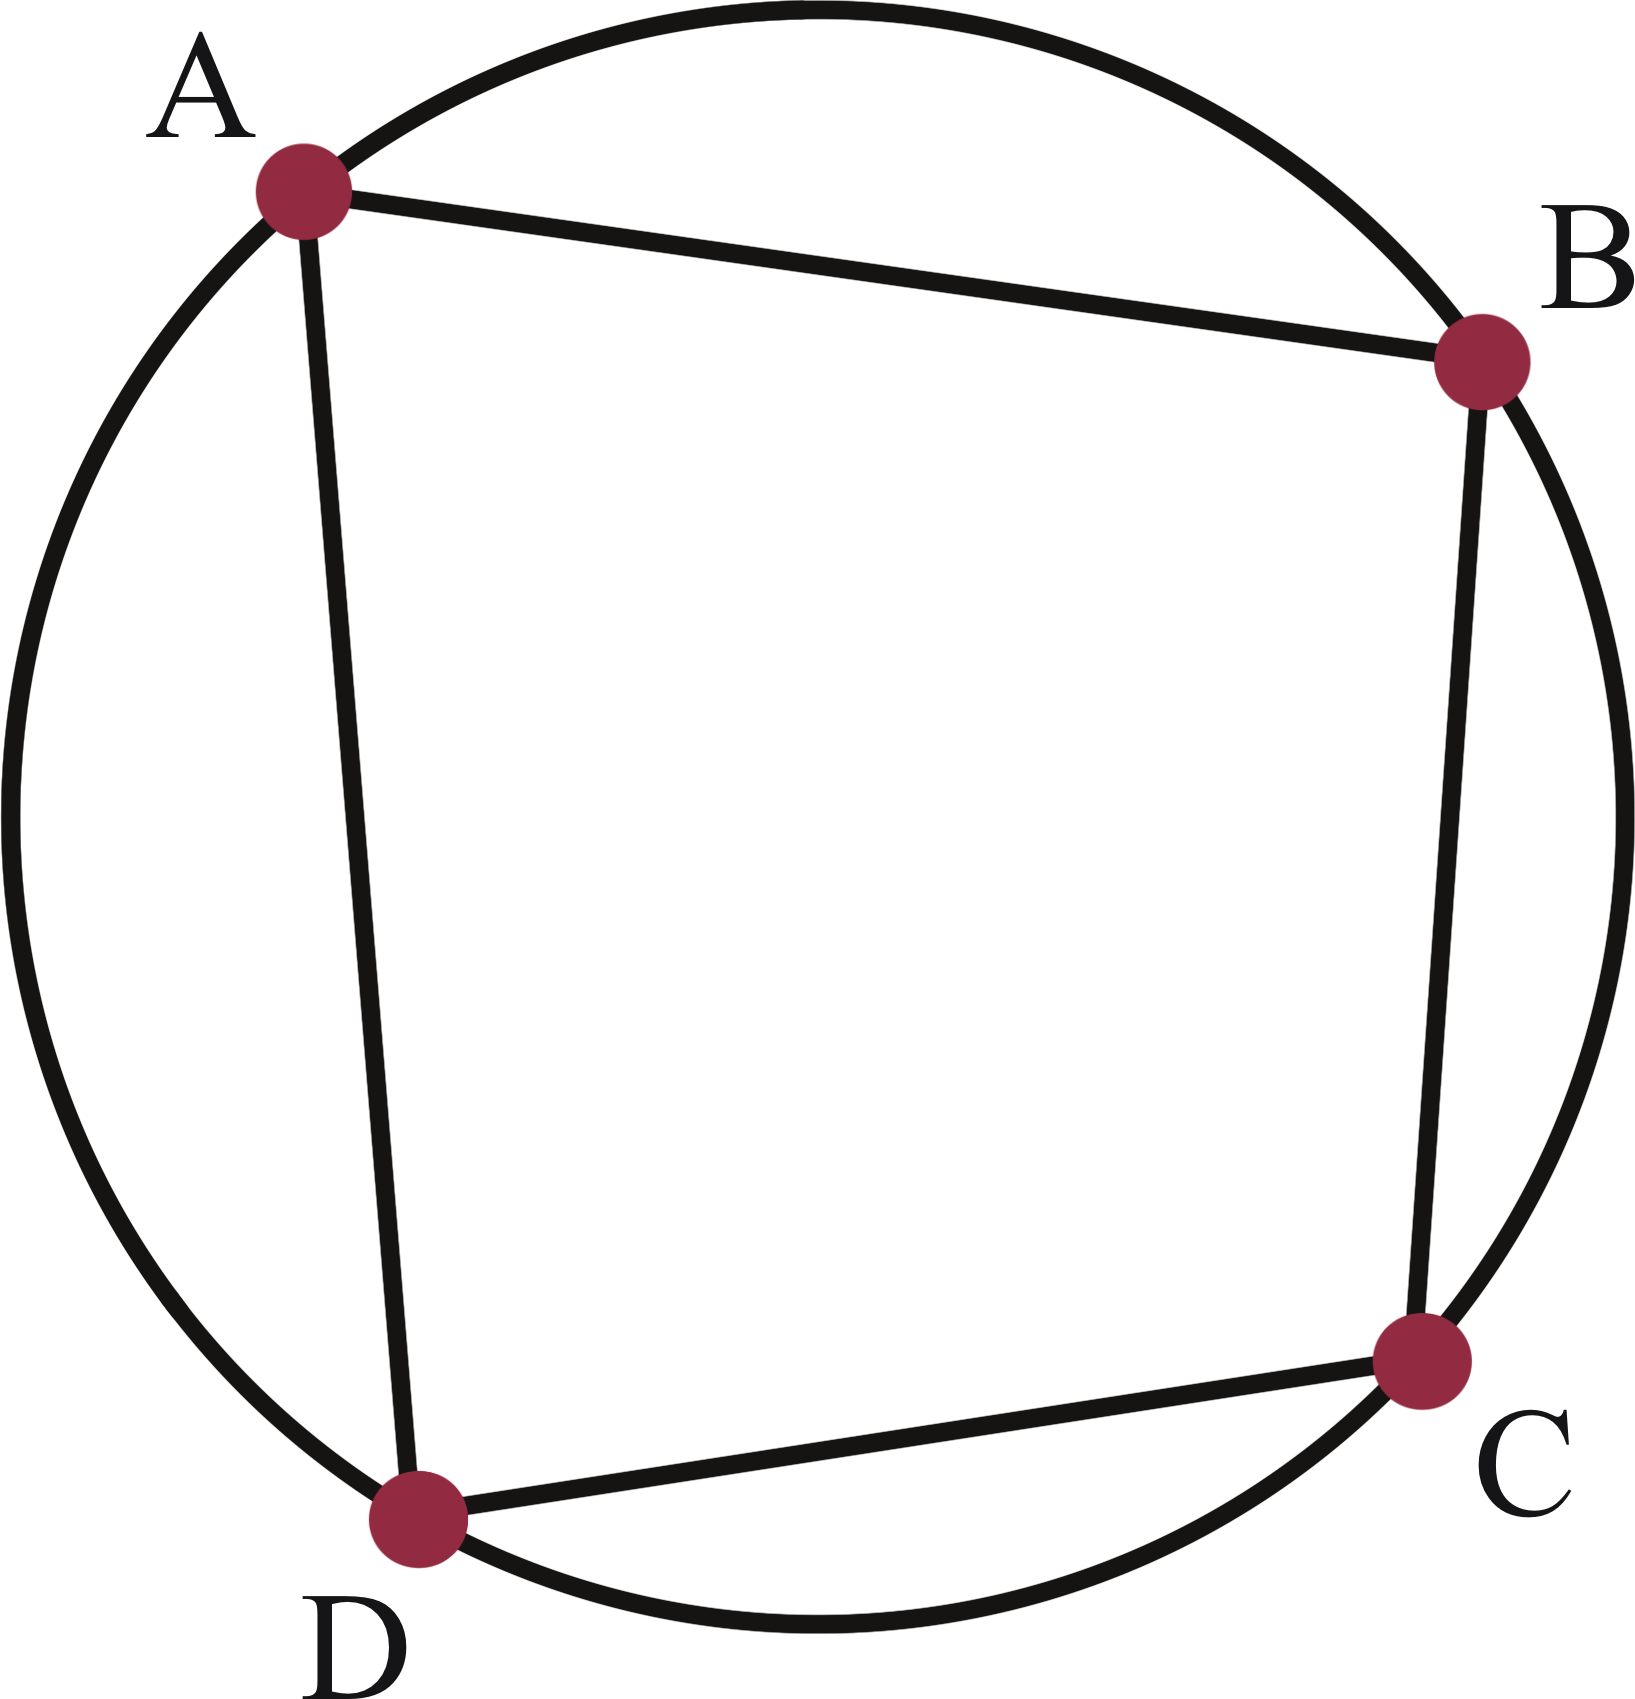
\includegraphics[width=\textwidth]{./ilustras-mat/Simulado_2-atividade_10_resposta.png}
\end{figure}

\item
SAEB: Reconhecer polígonos semelhantes ou as relações existentes
entre ângulos e lados correspondentes nesses tipos de polígonos.
BNCC: EF09MA12 -- Reconhecer as condições necessárias e suficientes para
que dois triângulos sejam semelhantes.
a) Correta. Para facilitar o entendimento, observe a figura a seguir.

\begin{figure}[htpb!]
\centering
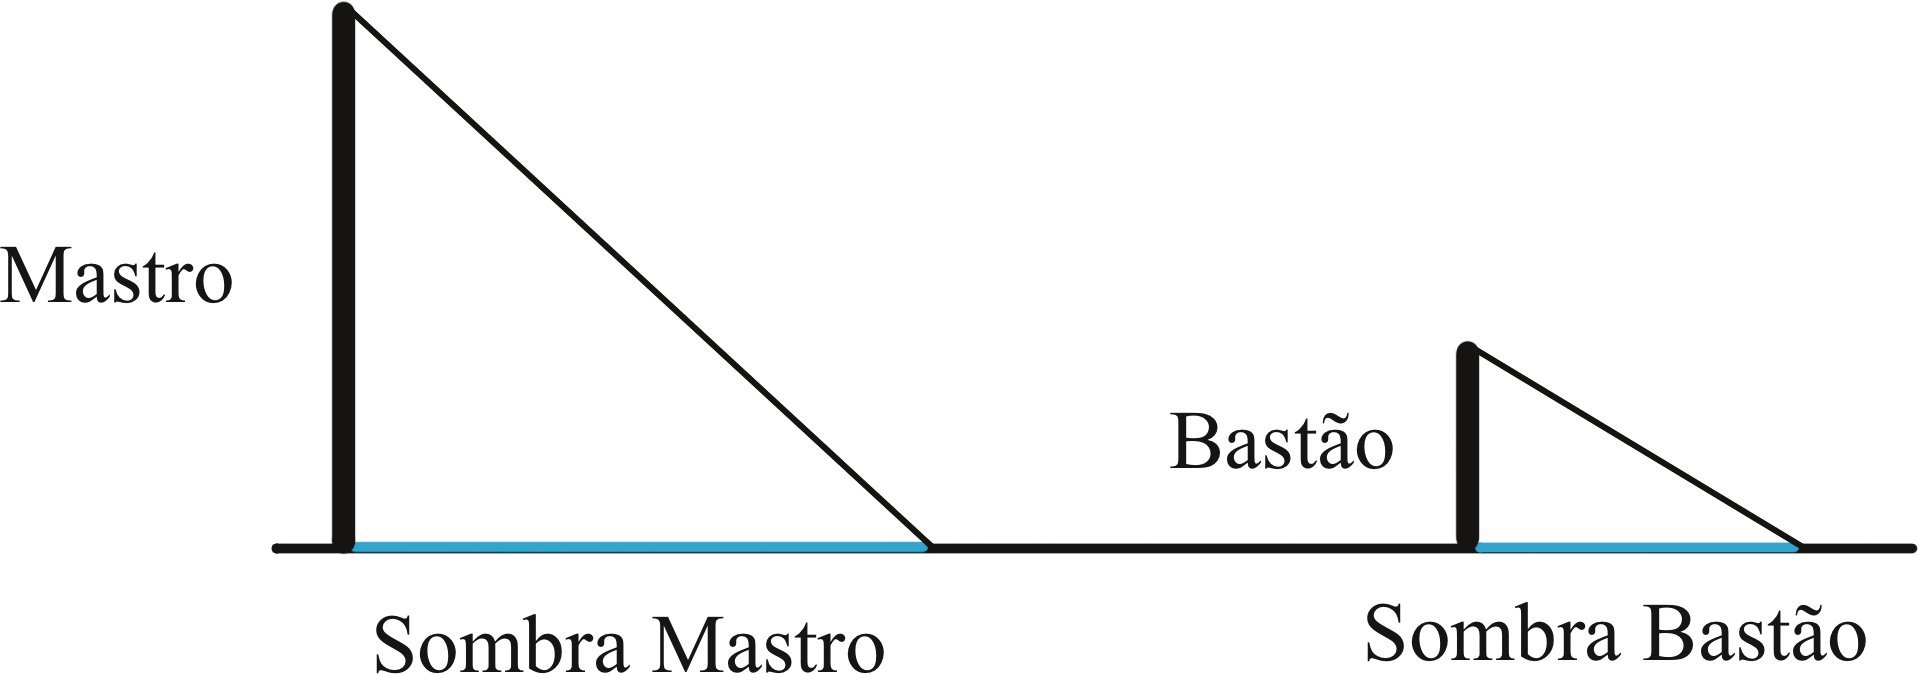
\includegraphics[width=\textwidth]{./ilustras-mat/Simulado_2-atividade_11.png}
\end{figure}


Dado que o momento da projeção das sombras do mastro e do bastão foi o
mesmo, pode-se afirmar que os triângulos são semelhantes. Dessa maneira, 
é possível calcular a razão entre as sombras e alturas.
Escrevendo todas as medidas em metros, obtém-se:

$\frac{1}{2,5} = \frac{x}{12,5} \rightarrow \\
x = \frac{12,5}{2,5} = 5$m.

b) Incorreta. A altura do mastro é de 5 metros.
c) Incorreta. A altura do mastro é de 5 metros.
d) Incorreta. A altura do mastro é de 5 metros.

\item
SAEB: Associar uma das representações de uma função afim ou
quadrática a outra de suas representações (tabular, algébrica, gráfica)
ou associar uma situação que envolva função afim ou quadrática a uma das
suas representações (tabular, algébrica, gráfica).
EF09MA06 -- Compreender as funções como relações de dependência unívoca
entre duas variáveis e suas representações numérica, algébrica e gráfica
e utilizar esse conceito para analisar situações que envolvam relações
funcionais entre duas variáveis.
a) Incorreta. A receita bruta foi de R\$ 9.000,00.
b) Correta. O dia com maior movimento naquela semana foi a quinta-feira,
na qual foram cobradas 450 corridas pela manhã e 300 à tarde. Dessa forma:
$(450 \cdot 10) + (300 \cdot 15) = 4500 + 4500 = 9000$. A receita bruta
foi, portanto, de R\$ 9.000,00.
c) Incorreta. A receita bruta foi de R\$ 9.000,00.
d) Incorreta. A receita bruta foi de R\$ 9.000,00.

\item
SAEB: Calcular os valores de medidas de tendência central de uma
pesquisa estatística (média aritmética simples, moda ou mediana).
BNCC: EF09MA21 -- Analisar e identificar, em gráficos divulgados pela mídia, os
elementos que podem induzir, às vezes propositadamente, erros de
leitura, como escalas inapropriadas, legendas não explicitadas
corretamente, omissão de informações importantes (fontes e datas), entre
outros.
a) Correta. Para atingir o objetivo do diretor financeiro, é necessário
que a mediana seja dada pela média aritmética entre R\$ 2000,00 e R\$ 
3600,00; para que isso ocorra, considerando demissões apenas de 
funcionários  que recebem 3600, o total de funcionários da empresa deve
ser igual a 22. Como, antes do corte, a empresa emprega 30 funcionários,
é necessário demitir 8 pessoas.
b) Incorreta. É necessário demitir 8 pessoas.
c) Incorreta. É necessário demitir 8 pessoas.
d) Incorreta. É necessário demitir 8 pessoas.

\item
SAEB: Resolver problemas que envolvam volume de prismas retos ou
cilindros retos.
BNCC: EF09MA19 -- Resolver e elaborar problemas que envolvam medidas de
volumes de prismas e de cilindros retos, inclusive com uso de expressões
de cálculo, em situações cotidianas.
a) Correta. Pode-se perceber que o bloco B possui 5 caixas de frente e 3
laterais: um total 15 vagas. Como são empilhadas 4 placas, uma sobre a
outra, são necessários 60 blocos de A para montar a pilha B.
b) Incorreta. São necessários 60 blocos de A para montar a pilha B.
c) Incorreta. São necessários 60 blocos de A para montar a pilha B.
d) Incorreta. São necessários 60 blocos de A para montar a pilha B.

\item
SAEB: Resolver problemas que envolvam relações métricas do
triângulo retângulo, incluindo o teorema de Pitágoras.
BNCC: EF09MA13 -- Demonstrar relações métricas do triângulo retângulo,
entre elas o teorema de Pitágoras, utilizando, inclusive, a semelhança
de triângulos.
a) Incorreta. A altura relativa à hipotenusa do triângulo é 4,8 cm.
b) Incorreta. A altura relativa à hipotenusa do triângulo é 4,8 cm.
c) Correta. É possível utilizar as relações métricas no triângulo
retângulo para determinar a altura relativa.
Pelo Teorema de Pitágoras, sabe-se que a hipotenusa vale 10, de modo que
se complementar a figura.
Usando a relação entre hipotenusa e altura: 

$10 \cdot h = 6 \cdot 8 \rightarrow h = 4,8$ cm.
d) Incorreta. A altura relativa à hipotenusa do triângulo é 4,8 cm.

\item
SAEB: Analisar as práticas corporais frente à disponibilidade de locais
para sua vivência.
BNCC: (EF89EF03):~formular e utilizar estratégias para solucionar os
desafios técnicos e táticos, tanto nos esportes de campo e taco,
rede/parede, invasão e combate como nas modalidades esportivas
escolhidas para praticar de forma específica.
a) Incorreta. Não há alusão, no texto, à ampliação de recursos financeiros do município associados ao uso da quadra. 
b) Correta. A quadra da escola Vinícius de Morais é utilizada 
primordialmente para aulas de educação física e práticas esportivas.  
c) Incorreta. Não há alusão, no texto, à promoção de competições oficiais de diferentes modalidades.
d) Incorreta. Nos fins de semana, a quadra pode abrigar atividades não esportivas, mas essa não é sua principal função.

\item
SAEB: Analisar as transformações históricas, o processo de
esportivização e a midiatização das práticas corporais, com ênfase nas
lutas.
BNCC: (EF89EF18): Discutir as transformações históricas, o processo de
esportivização e a midiatização de uma ou mais lutas, valorizando e
respeitando as culturas de origem.
a) Incorreta. A prática centenária da esgrima não é condição suficiente 
para que essa prática seja considerada esporte oficial.
b) Correta. A regulação por federações ou confederações caracteriza a 
esgrima como esporte oficial. 
c) Incorreta. A origem bélica da esgrima não é condição suficiente 
para que essa prática seja considerada esporte oficial. 
d) Incorreta. O uso de instrumento específico, como a espada, não é
condição suficiente  para que essa prática seja considerada esporte 
oficial.

\item
SAEB: Diferenciar os esportes com base nos critérios de sua lógica
interna.
BNCC: EF67EF13 -- Diferenciar as danças urbanas das demais manifestações
da dança, valorizando e respeitando os sentidos e significados
atribuídos a eles por diferentes grupos sociais.
a) Incorreta. A cultura hip hop deu origem ao Breaking Dance e outras
práticas corporais.
b) Correta. Pode-se afirmar que o Breaking Dance tornou-se esporte
porque será disputado em competição oficial. 
c) Incorreta. O autor do texto não menciona que o Breaking Dance tenha
incentivado competições de dança.
d) Incorreta. O Breaking Dance preserva as características de dança
urbana, mesmo que suas regras tenham sido padronizadas para as Olimpíadas.

\item
BNCC: EF09CI02 - Comparar quantidades de reagentes e
produtos envolvidos em transformações químicas, estabelecendo a
proporção entre as suas massas.
a)  Incorreta. A Inércia, também conhecida como primeira lei de Newton,
  não diz respeito à conservação das massas em uma reação.
b)  Incorreta. A lei da proporção fala da composição das substâncias envolvidas em uma reação.
c)  Incorreta. A lei de Gay-Lussac, além de não ser proposta por Lavoisier, trata das condições que influenciam uma reação, como pressão e temperatura.
d)  Correta. A Lei de Lavoisier é justamente a Lei de conservação das
  massas, que considera que a massa dos reagentes deve ser igual à massa do produto.

\item
BNCC: EF09CI11 -- Discutir a evolução e a diversidade
das espécies com base na atuação da seleção natural sobre as variantes
de uma mesma espécie, resultantes de processo reprodutivo.
a) Correta. Ao dizimar populações, o fungo reduz a riqueza de espécies de anfíbios, ou seja, afeta a biodiversidade da área. Além disso, 
impacta o equilíbrio do ecossistema, pois anfíbios servem de alimento
para outros animais, comem artrópodes e controlam comunidades de invertebrados.
b) Incorreta. A evolução é um processo constante e atemporal, portanto, acontecerá independentemente das imprevisibilidades existentes
dentro de um ecossistema, como a endemia citada.
c) Incorreta. O texto-base comenta que os fungos começam a ameaçar também sapos que habitam o ambiente terrestre; portanto, esses organismos serão afetados independentemente do seu modo de reprodução.
d) Incorreta. A alternativa faz alusão à teoria evolucionista
pensada por Lamarck, que não é adotada atualmente e afirma que os seres
vivos se modificam para sobreviver no ambiente.

\item
BNCC: EF09CI17 -- Analisar o ciclo evolutivo do Sol
(nascimento, vida e morte) baseado no conhecimento das etapas de
evolução de estrelas de diferentes dimensões e os efeitos desse processo
no nosso planeta.
a)  Correta. A força gravitacional de um buraco negro atrairia a
  Terra com tanta intensidade que toda a matéria da Terra se separaria
  em pequenas partículas e o tempo passaria extremamente lento.
b)  Incorreta. Mesmo sendo bastante pequena em comparação a um buraco
  negro, a Terra seria engolida e destruída por ele.
c)  Incorreta. No encontro de duas galáxias as condições seriam
  catastróficas e o buraco negro formado pelo encontro do centro dessas
  galáxias seria gigantesco; dessa forma a força gravitacional da Terra seria imperceptível.
d) Incorreta. A força gravitacional do buraco negro tende a puxar os corpos para si, engolindo a Terra, mesmo com a existência do efeito
  estilingue que acontece na borda de um buraco negro.
\end{enumerate}

\colorsec{Simulado 3}

\begin{enumerate}
\item
SAEB: Identificar números racionais ou irracionais. 
EF09MA02 - Reconhecer um número irracional como um número real cuja
representação decimal é infinita e não periódica, e estimar a localização
de alguns deles na reta numérica. 

O número $\sqrt{8} + \sqrt{18}$ pode ser escrito como $5\sqrt{2}$.

a) Incorreta. O número $\sqrt{8} + \sqrt{18}$ pode ser escrito 
como $5\sqrt{2}$. 
b) Incorreta. O número $\sqrt{8} + \sqrt{18}$ pode ser escrito 
como $5\sqrt{2}$. 
c) Correta. $\sqrt{8} + \sqrt{18} = \sqrt{2^{2} \cdot 2} + \sqrt{3^{2} \cdot 2} = 2\sqrt{2} + 3\sqrt{2} = 5\sqrt{2}.$
d) Incorreta. O número $\sqrt{8} + \sqrt{18}$ pode ser escrito 
como $5\sqrt{2}$.

\item
SAEB Resolver problemas de adição, subtração, multiplicação, divisão, potenciação ou radiciação envolvendo números reais, inclusive notação científica.
EF09MA03 -- Efetuar cálculos com números reais, inclusive potências com
expoentes fracionários.
a) Incorreta. Existem 500 resmas na distribuidora.
b) Incorreta. Existem 500 resmas na distribuidora.
c) Incorreta. Existem 500 resmas na distribuidora.
d) Correta. Cada pilha tinha 1 m = 1.000 mm. O número de folhas em
uma pilha é calculado pela divisão entre 1.000 por 0,4 mm.
$\frac{1000}{0,4} = 2500$. Calculando $100 \cdot 2.500 = 250.000$ folhas.
Como cada resma tem 500 folhas, basta dividir 250.000 folhas por 500
folhas. $\frac{250.000}{500} = 500$ resmas.

\item
SAEB: Determinar uma fração geratriz para uma dízima periódica.
a) Incorreta. O valor de $x + y = \frac{82}{99}$.
b) Incorreta. O valor de $x + y = \frac{82}{99}$.
c) Correta. Primeiramente escreve-se a fração geratriz de cada número:

$0,27272727\ldots{} = \frac{27}{99}$ e $0,5555\ldots{} = \ \frac{5}{9}$

Agora pode-se fazer a soma:

$\frac{27}{99} + \frac{5}{9} = \frac{27 + 55}{99} = \frac{82}{99}$.

d) Incorreta. O valor de $x + y = \frac{82}{99}$.

\item
SAEB: Resolver problemas que envolvam porcentagens, incluindo os
que lidam com acréscimos e decréscimos simples, aplicação de percentuais
sucessivos e determinação das taxas percentuais.
BNCC: EF09MA05 -- Resolver e elaborar problemas que envolvam
porcentagens, com a ideia de aplicação de percentuais sucessivos e a
determinação das taxas percentuais, preferencialmente com o uso de
tecnologias digitais, no contexto da educação financeira.
a) Incorreta. O valor a ser pago será de R\$ 300,00.
b) Incorreta. O valor a ser pago será de R\$ 300,00.
c) Correta. Para determinar o resultado, precisamos apenas calcular 
25\% de 400: $0,25 \cdot 400 = 100$. Como o desconto será de R\$100,00, 
o valor a ser pago será de R\$ 300,00.
d) Incorreta. O valor a ser pago será de R\$ 300,00.

\item
SAEB: Resolver uma equação polinomial de 1º grau
a) Incorreta. Cada caixa pequena tem 100 gramas.
b) Correta. Seja x a massa da caixa, temos:

$300 + 3x = 600$ \\

$3x = 300$ \\

$x = 100$. Cada caixa pequena tem, portanto, 100 gramas.
c) Incorreta. Cada caixa pequena tem 100 gramas.
d) Incorreta. Cada caixa pequena tem 100 gramas.

\item
SAEB: Identificar uma representação algébrica para o padrão ou
a regularidade de uma sequência de números racionais OU representar
algebricamente o padrão ou a regularidade de uma sequência de números
racionais.
a) Incorreta. A relação entre y e x é dada pela expressão $y = 4x - 3$.
b) Incorreta. A relação entre y e x é dada pela expressão $y = 4x - 3$.
c) Correta. Observando os valores de y, pode-se perceber que o aumento 
de y a cada unidade aumentada em x é 4, de modo que verifica-se que a
expressão será 4x com algum ajuste. Fazendo $4 \cdot 5$ obtém-se 20, mas o 
número é 17 (3 a menos); fazendo $4 \cdot 6$ obtém-se 24, mas o número é 21
(3 a menos), logo é possível afirmar que $y = 4x - 3$. A relação entre y e
x, portanto, é dada pela expressão $y = 4x - 3$.
d) Incorreta. A relação entre y e x é dada pela expressão $y = 4x - 3$.

\item
SAEB: 9A1.7 - Resolver uma equação polinomial de 2º grau.

a) Incorreta. As raízes da equação são - 6 e 4, valores compreendidos no 
intervalo de --7 até 5.
b) Correta. Para resolver essa equação, é possível utilizar a fórmula de Bhaskara.

$\Delta = 2^{2} - 4 \cdot 1 \cdot (24) = 4 + 96 = 100$

$x = \frac{-2 \pm \sqrt{100}}{2 \cdot 1} = \frac{- 2 \pm 10}{2} =$

%\left\{\begin{matrix}
$\frac{-2+10}{2} = 4$

$\frac{-2-10}{2} = -6 $
%\end{matrix}\right$

As raízes da equação são - 6 e 4, valores compreendidos no intervalo 
de --7 até 5.
c) Incorreta. As raízes da equação são - 6 e 4, valores compreendidos no 
intervalo de --7 até 5.
d) Incorreta. As raízes da equação são - 6 e 4, valores compreendidos no 
intervalo de --7 até 5.

\item
SAEB: Resolver problemas que envolvam variação de
proporcionalidade direta ou inversa entre duas ou mais grandezas,
inclusive escalas, divisões proporcionais e taxa de variação.
BNCC: EF09MA08 -- Resolver e elaborar problemas que envolvam relações de
proporcionalidade direta e inversa entre duas ou mais grandezas,
inclusive escalas, divisão em partes proporcionais e taxa de variação,
em contextos socioculturais, ambientais e de outras áreas.
a) Correta. Se $40 m^2$ foram trabalhados em 80 minutos, numa relação de
$\frac{1}{2}$, mantém-se a mesma proporção para os $160 m^2$, que serão
trabalhados em 320 minutos. 
b) Incorreta. Serão gastos 320 minutos para concluir o trabalho. 
c) Incorreta. Serão gastos 320 minutos para concluir o trabalho. 
d) Incorreta. Serão gastos 320 minutos para concluir o trabalho.

\item
SAEB: Resolver problemas que envolvam função afim.
BNCC: EF09MA06 -- Compreender as funções como relações de dependência
unívoca entre duas variáveis e suas representações numérica, algébrica e
gráfica e utilizar esse conceito para analisar situações que envolvam
relações funcionais entre duas variáveis.
Ao final de 30 minutos havia 117 vírus.

a) Incorreta. Ao final de 30 minutos havia 117 vírus.
b) Correta. Dada a regularidade de aumento de 4 vírus a cada 1 minuto, obtém-se 
a expressão do tipo $q = 4n + k$. Como para 3 minutos há
9 vírus, pode-se determinar k, pois: 

$9 = 4 \cdot3 + k \\
9 - 12 = k \\ 
k = - 3$.

Dado que $q = 4n - 3 \rightarrow q = 4 \cdot30 - 3 = 120 - 3 = 117$.
c) Incorreta. Ao final de 30 minutos havia 117 vírus.
d) Incorreta. Ao final de 30 minutos havia 117 vírus.

\item
SAEB: Resolver problemas que envolvam polígonos semelhantes.
Resolver problemas que envolvam área de figuras planas.
BNCC: -- Reconhecer as condições necessárias e suficientes para
que dois triângulos sejam semelhantes.

a) Incorreta. A área é igual a $4,8^2 = 23,04$ unidade de medida quadrada.
b) Incorreta. A área é igual a $4,8^2 = 23,04$ unidade de medida quadrada. 
c) Incorreta. A área é igual a $4,8^2 = 23,04$ unidade de medida quadrada. 
d) Correta. $\frac{8 - x}{x} = \frac{x}{12 - x} \rightarrow x^{2} = 96 - 8x - 12x + x^2 \rightarrow 20x = 96 \rightarrow x = 4,8$.

A área é igual a $4,8^2 = 23,04$ unidade de medida quadrada.

\item
SAEB: Resolver problemas que envolvam relações métricas do
triângulo retângulo, incluindo o teorema de Pitágoras.
BNCC: EF09MA13 -- Demonstrar relações métricas do triângulo retângulo,
entre elas o teorema de Pitágoras, utilizando, inclusive, a semelhança
de triângulos.
a) Correta. Calculando o valor do cateto utilizando o Teorema de 
Pitágoras: $13^2 = 5^2 + x^2 \rightarrow 169 - 25 = x^2 \rightarrow x = 12 cm$.
b) Incorreta. O outro cateto mede 12 cm.
c) Incorreta. O outro cateto mede 12 cm.
d) Incorreta. O outro cateto mede 12 cm.

\item
SAEB: 9E2.2 - Argumentar ou analisar argumentações/conclusões com base
nos dados apresentados em tabelas (simples ou de dupla entrada) ou
gráficos (barras simples ou agrupadas, colunas simples ou agrupadas,
pictóricos, de linhas, de setores ou em histograma).
BNCC: EF09MA21 - Analisar e identificar, em gráficos divulgados pela
mídia, os elementos que podem induzir, às vezes propositadamente, erros
de leitura, como escalas inapropriadas, legendas não explicitadas
corretamente, omissão de informações importantes (fontes e datas), entre
outros.
a) Incorreta. Em 2021 ocorreu crescimento linear das vendas, mês a mês.
b) Incorreta. Em 2022, de julho para agosto, houve aumento das vendas.
c) Correta. De fato, houve queda nas vendas do mês de setembro para 
o de outubro em 2022 
d) Incorreta. Entre novembro e dezembro de 2022 as vendas ficaram 
estáveis.

\item
SAEB: Calcular os valores de medidas de tendência central de uma
pesquisa estatística (média aritmética simples, moda ou mediana).
BNCC: EF09MA21 -- Analisar e identificar, em gráficos divulgados pela
mídia, os elementos que podem induzir, às vezes propositadamente, erros
de leitura, como escalas inapropriadas, legendas não explicitadas
corretamente, omissão de informações importantes (fontes e datas), entre
outros.
a) Correta. A moda é o valor mais frequente de um conjunto de dados. Para
encontrá-la basta observar o dado mais frequente que, no caso, é o número
2, que saiu 21 vezes.
b) Incorreta. A moda dos resultados é 2.
c) Incorreta. A moda dos resultados é 2.
d) Incorreta. A moda dos resultados é 2.

\item
SAEB: Resolver problemas que envolvam porcentagens, incluindo os
que lidam com acréscimos e decréscimos simples, aplicação de percentuais
sucessivos e determinação de taxas percentuais.
BNCC: EF09MA05 -- Resolver e elaborar problemas que envolvam
porcentagens, com a ideia de aplicação de percentuais sucessivos e a
determinação das taxas percentuais, preferencialmente com o uso de
tecnologias digitais, no contexto da educação financeira.
a) Incorreta. O valor da parcela é de R\$ 630.
b) Incorreta. O valor da parcela é de R\$ 630.
c) Incorreta. O valor da parcela é de R\$ 630.
d) Correta. Calculando 30\% de 4.500 encontramos o valor de 1.350,00. O 
saldo estante é R\$ 3.150,00, de modo que a parcela será igual 
$3150 \div 5 = 630$. Serão cobradas, portanto, 5 parcelas de R\$ 630,00.

\item
SAEB: Resolver problemas que envolvam a probabilidade de
ocorrência de um resultado em eventos aleatórios equiprováveis
independentes ou dependentes.
BNCC: EF09MA20 -- Reconhecer, em experimentos aleatórios, eventos
independentes e dependentes e calcular a probabilidade de sua
ocorrência, nos dois casos.
a) Incorreta. A probabilidade de que a soma dos resultados seja 
7 é $\frac{1}{6}$.
b) Incorreta. A probabilidade de que a soma dos resultados seja 
7 é $\frac{1}{6}$.
c) Incorreta. A probabilidade de que a soma dos resultados seja 
7 é $\frac{1}{6}$.
d) Correta. Para facilitar a contagem podemos montar uma tabela com as 36
possibilidades de resultados do lançamento de 2 dados:

\begin{longtable}[]{@{}lllllll@{}}
\toprule
\textbf{~} & \textbf{1} & \textbf{2} & \textbf{3} & \textbf{4} &
\textbf{5} & \textbf{6}\tabularnewline
\midrule
\endhead
\textbf{1} & \textbf{~} & \textbf{~} & \textbf{~} & \textbf{~} &
\textbf{~} & \textbf{~}\tabularnewline
\textbf{2} & \textbf{~} & \textbf{~} & \textbf{~} & \textbf{~} &
\textbf{~} & \textbf{~}\tabularnewline
\textbf{3} & \textbf{~} & \textbf{~} & \textbf{~} & \textbf{~} &
\textbf{~} & \textbf{~}\tabularnewline
\textbf{4} & \textbf{~} & \textbf{~} & \textbf{~} & \textbf{~} &
\textbf{~} & \textbf{~}\tabularnewline
\textbf{5} & \textbf{~} & \textbf{~} & \textbf{~} & \textbf{~} &
\textbf{~} & \textbf{~}\tabularnewline
\textbf{6} & \textbf{~} & \textbf{~} & \textbf{~} & \textbf{~} &
\textbf{~} & \textbf{~}\tabularnewline
\bottomrule
\end{longtable}

Marcando as possibilidades de soma igual a 7, encontramos 6 situações.
Então a probabilidade de encontrar a soma 7 temos:

$P(A) = \frac{6}{36} = \frac{1}{6}$.

\item
SAEB: Diferenciar as danças urbanas, seus elementos constitutivos
e seu valor cultural nas demais manifestações da dança.
BNCC: EF67EF12 -- Planejar e utilizar estratégias para aprender
elementos constitutivos das danças urbanas.
a) Incorreta. O autor do texto não menciona o incentivo a práticas
esportivas como propósito da cultura hip hop. 
b) Incorreta. Não há referências, no texto, ao estímulo do empreendedorismo
social como propósito da cultura hip hop. 
c) Incorreta. A redução da violência por meio da arte não é mencionada, no 
texto, como propósito primordial do hip hop. 
d) Correta. Segundo o autor, o hip hop surgiu como forma de contestação 
das comunidades caribenhas, afro-americanas e latino-americanas na
década de 1970.

\item
SAEB: Avaliar a multiplicidade de padrões de estética corporal
disseminados pela mídia, que geram uma prática excessiva de exercícios e
o uso de recursos ergogênicos
BNCC: EF89EF08 -- Discutir as transformações históricas dos padrões de
desempenho, saúde e beleza, considerando a forma como são apresentados
nos diferentes meios (científico, midiático, etc.).
a) Incorreta. A obsessão pela alimentação saudável caracteriza a ortorexia. 
b) Correta. A vigorexia é um transtorno no qual o indivíduo
tem de si mesmo uma imagem distorcida: embora tenha compleição
física forte e musculosa, diante do espelho ele se vê como fraco
e franzino. Por causa dessa distorção, ele insiste na prática de 
exercícios físicos em excesso, com a finalidade de obter a imagem 
de força.
c) Incorreta. A indução do vômito após uma refeição é comportamento típico de pessoas acometidas pela bulimia. 
d) Incorreta. A ingestão de pequenas quantidades de alimentos é comportamento típico de pessoas acometidas pela anorexia.

\item
SAEB: Avaliar os problemas presentes nos esportes e abordados pela
mídia, tais como doping, violência ou corrupção.
BNCC: EF89EF09 -- Problematizar a prática excessiva de exercícios
físicos e o uso de medicamentos para a ampliação do rendimento ou
potencialização das transformações corporais.
a) Incorreta. Atletas que evitam o uso de substâncias ilegais se afastam
da prática do \textit{doping}.
b) Correta. A alternativa corrobora a definição de \textit{doping} 
apresentada no texto. 
c) Incorreta. A prática do \textit{doping} não está associada a 
tratamentos médicos, mas à melhora do desempenho dos atletas em 
competições.
d) Incorreta. A prática do \textit{doping} não está associada
a cuidades de saúde,mas à melhora do desempenho dos atletas em 
competições.

\item
BNCC: EF09CI03 -- Identificar modelos que descrevem
a estrutura da matéria (constituição do átomo e composição de moléculas
simples) e reconhecer sua evolução histórica.
a)  Incorreta. O processo de liofilização consiste na retirada de água de
  uma substância; elétrons não têm água.
b)  Incorreta. Os elétrons são tão pequenos que não são captados pelas
  ondas luminosas e, dessa forma, são invisíveis para a luz.
c)  Correta. A ionização, ou seja, a doação de cargas faz com que os
  elétrons se excitem e se movimentem pelos átomos.
d)  Incorreta. O processo de centrifugação consiste em agitar substâncias
  a fim de apressar o processo de decantação, o que não faz sentido para
  elétrons.

\item
BNCC: EF09CI12 -- Justificar a importância das
unidades de conservação para a preservação da biodiversidade e do
patrimônio nacional, considerando os diferentes tipos de unidades
(parques, reservas e florestas nacionais), as populações humanas e as
atividades a eles relacionados.
a)  Correta. A construção de corredores ecológicos, se feita sob um
  estudo e com planejamento, visa a preservar a possibilidade de locomoção
  de animais, bem como a passagem de rodovias para a circulação de seres humanos.
b)  Incorreta. As opções de locomoção por vias aquáticas e aéreas também geram
  impactos ambientais e colocam em risco a vida de animais, além de
  serem menos vantajosas para viagens dentro do País.
c)  Incorreta. Isolar cidades e comunidades limitaria o acesso dos moradores à educação, à saúde e até à alimentação.
d)  Incorreta. Cobrar taxas de circulação não garante que vá haver
  manutenção e proteção da biodiversidade presente no local.

\item
BNCC: EF09CI14 -- Descrever a composição e a
estrutura do Sistema Solar (Sol, planetas rochosos, planetas gigantes
gasosos e corpos menores), assim como a localização do Sistema Solar na
nossa Galáxia (a Via Láctea) e dela no Universo (apenas uma galáxia
dentre bilhões).
a)  Incorreta. Não há possibilidades de o Sol ficar entre a Terra e a
  Lua por conta dos seus tamanhos, distâncias e órbitas.
b)  Correta. Em um eclipse solar a Lua fica entre o Sol e a Terra, evitando que a luz solar chegue completamente a alguns pontos da Terra.
c)  Incorreta. Não há possibilidades de Marte passar entre o Sol e a
  Terra, já que Marte se encontra mais distante do Sol do que a própria Terra.
d)  Incorreta. Quando a Terra se encontra entre a Lua e o Sol temos um eclipse lunar.

\end{enumerate}

\colorsec{Simulado 4}

\begin{enumerate}
\item
SAEB - 9N1.3 - números racionais ou irracionais.
EF09MA02 - Reconhecer um número irracional como um número real cuja
representação decimal é infinita e não periódica, e estimar a
localização de alguns deles na reta numérica.
$\sqrt{12} = 2\sqrt{3}$ é um número irracional, pois não é possível
escrever este número em forma de fração.

\item
SAEB -- 9N2.1 - Resolver problemas de adição, subtração, multiplicação,
divisão, potenciação ou radiciação envolvendo números reais,
EF09MA03 - Efetuar cálculos com números reais, inclusive potências com
expoentes fracionários.
Alternativa

$V = \frac{9,45 \cdot 10^{15}}{3,15 \cdot 10^{7}} = 3 \cdot 10^{8}m/s$\emph{.}

\item
SAEB 9N1.8 -- Identificar frações equivalentes. Escrevendo 37,5\% em
forma de fração irredutível, temos:
$37,5\% = \frac{37,5}{100} = \frac{375}{1000} = \frac{3}{8}$, ou seja,
temos exatamente o mesmo valor representado. Alternativa a.

\item
SAEB: 9N2.3 - Resolver problemas que envolvam porcentagens, incluindo os
que lidam com acréscimos e decréscimos simples, aplicação de percentuais
sucessivos e determinação das taxas percentuais.

Podemos determinar o valor antes do aumento verificando qual foi o
percentual total aplicado. Para isso usaremos o fator de correção (1+i)
= (1 + 0,08) e (1+0,12). Foram dois aumentos sucessivos, sendo assim:
$\left( 1 + 0,08 \right) \cdot \left( 1 + 0,12 \right) = 1,2026$, ou
seja, o valor de 60,48 representa 120,96\% do preço inicial.

Preço \%

X 100

60,48 120,96

Resolvendo a regra de três, temos: $\frac{6048}{120,96} = 50$.

Ou seja, antes do aumento a mercadoria custava R\$ 50,00. Alternativa a.

\item
SAEB: 9A1.1 - Resolver uma equação polinomial de 1º grau.

Seja x o número de sobrinhos, sendo assim temos: 8x + 44 = 10x -- 12.

$$8x -- 10x = -- 12 -- 44 → -- 2x = -- 56 → x = 28.$$

Alternativa d.

\item
SAEB: 9A2.2 - Resolver problemas que envolvam cálculo do valor numérico
de expressões algébricas.
Fazendo a substituição temos q = 8 \cdot (8 + 1) = 8 \cdot 9 = 72.
Alternativa d.

\item
SAEB: 9A1.7 - Resolver uma equação polinomial de
2º grau. Para determinar a quantidade de lados, precisamos resolver a
equação: $14 = \frac{n^{2} - 3n}{2} \rightarrow n^{2} - 3n - 28 = 0$,
por se tratar de uma equação do 2º grau podemos aplicar Bhaskara.

\[\mathrm{\Delta} = \left( - 3 \right)^{2} - 4 \cdot 1 \cdot \left( - 28 \right) = 9 + 112 = 121\]

$n = \frac{- ( - 3) \pm \sqrt{121}}{2} = \frac{3 \pm 11}{2} = \left\{ \begin{matrix} \frac{3 + 11}{2} = 7\ \ \ \ \ \ \ \ \ \ \ \ \ \ \ \ \ \ \ \ \ \ \ \ \ \ \ \ \ \  \\ \frac{3 - 11}{2} = - 4\ Não\ convém \\ \end{matrix} \right.\ $.
Por se tratar de quantidade de lados de um polígono desprezamos o valor
negativo. Alternativa d.

\item
SAEB: 9A2.1 - Resolver problemas que envolvam variação de
proporcionalidade direta ou inversa entre duas ou mais grandezas,
inclusive escalas, divisões proporcionais e taxa de variação.
BNCC: EF09MA08 - Resolver e elaborar problemas que envolvam relações de
proporcionalidade direta e inversa entre duas ou mais grandezas,
inclusive escalas, divisão em partes proporcionais e taxa de variação,
em contextos socioculturais, ambientais e de outras áreas.
Proporcionalmente se a cada 100 gramas obtemos 24 gramas de açúcar, em
400 gramas teremos 96 gramas (4 \cdot 24 = 96). Podemos ainda concluir que
em 50 gramas teremos 12 gramas de açúcar, pois é metade da massa
descrita na etiqueta, sendo assim em 450 gramas teremos 96 + 12 = 108
gramas de açúcar.
Alternativa c.

\item
SAEB: 9A1.3 - Identificar uma representação algébrica para o padrão ou a
regularidade de uma sequência de números racionais ou representar
algebricamente o padrão ou a regularidade de uma sequência de números
racionais.

\item
SAEB: 9G2.5 - Resolver problemas que envolvam polígonos semelhantes.
BNCC: EF09MA12 - Reconhecer as condições necessárias e suficientes para
que dois triângulos sejam semelhantes.
$\frac{x}{12} = \frac{3}{x} \rightarrow x^{2} = 36 \rightarrow x = 6$.
Alternativa c.

\item
SAEB: 9E2.2 - Argumentar ou analisar argumentações/conclusões com base
nos dados apresentados em tabelas (simples ou de dupla entrada) ou
gráficos (barras simples ou agrupadas, colunas simples ou agrupadas,
pictóricos, de linhas, de setores ou em histograma).
BNCC: EF09MA22 - Escolher e construir o gráfico mais adequado (colunas,
setores, linhas), com ou sem uso de planilhas eletrônicas, para
apresentar um determinado conjunto de dados, destacando aspectos como as
medidas de tendência central.

\item
SAEB: 9M2.4 - Resolver problemas que envolvam volume de prismas retos ou
cilindros retos.
BNCC: EF09MA19 - Resolver e elaborar problemas que envolvam medidas de
volumes de prismas e de cilindros retos, inclusive com uso de expressões
de cálculo, em situações cotidianas.

$V_{1} = \pi \cdot 6^{2} \cdot 4 = 144\pi$ →
$V_{2} = \pi \cdot 3^{2} \cdot x$ →
$\pi \cdot 3^{2} \cdot x = 144\pi \rightarrow x = 16.$

Alternativa c.

\item
SAEB: 9E1.5 - Calcular os valores de medidas de tendência central de uma
pesquisa estatística (média aritmética simples, moda ou mediana).
Para determinar a mediana precisamos colocar os número em ordem:
6,8 7,2 7,2 8,4 8,7 9,1

A mediana é calculada como média aritmética entre 7,2 e 8,4:
$\frac{7,2 + 8,4}{2} = \frac{15,6}{2} = 7,8$. A média é :
$\frac{6,8 + 7,2 + 7,2 + 8,4 + 8,7 + 9,1}{6} = 7,9$.

Alternativa a.

\item
SAEB: 9M2.4 - Resolver problemas que envolvam volume de prismas retos ou
cilindros retos.
BNCC: EF09MA19 - Resolver e elaborar problemas que envolvam medidas de
volumes de prismas e de cilindros retos, inclusive com uso de expressões
de cálculo, em situações cotidianas.
Volume da caixa cúbica: V\textsubscript{Caixa} = 1m³
Volume do cano: V\textsubscript{Cano} = (0,02)² \cdot 3,14 \cdot 50 = 0,0628 m³
Volume total: 1,0628 m³ = 1 062,8 litros.
Alternativa c.

\item
SAEB: 9E2.4 - Resolver problemas que envolvam a probabilidade de
ocorrência de um resultado em eventos aleatórios equiprováveis
independentes ou dependentes.
BNCC: EF09MA20 - Reconhecer, em experimentos aleatórios, eventos
independentes e dependentes e calcular a probabilidade de sua
ocorrência, nos dois casos.
A probabilidade de que os números sejam diferentes é igual a
$\frac{21}{28} = 0,75 = 75\%.$

\item
SAEB: Avaliar a relação entre as práticas corporais e a promoção da
saúde.
BNCC: EF89EF08) -- Discutir as transformações históricas dos padrões de
desempenho, saúde e beleza, considerando a forma como são apresentados
nos diferentes meios (científico, midiático, etc.).
a) Incorreta. As atividades físicas devem ser preticadas em todas as
fases da vida. 
b) Correta. As atividades físicas previnem ocorrências de Doenças Crônicas Não Transmissíveis.
c) Correta. As atividades físicas trazem benefícios para as pessoas, 
em termos individuais, e para a sociedade como um todo.
d) Incorreta. As atividades físicas são benéficas para a saúde física e
psicológica.

\item
SAEB: Identificar as diferentes valências físicas necessárias à
realização de práticas corporais (jogos eletrônicos, lutas, práticas
corporais de aventura, ginásticas, esportes e dança).
BNCC: EF67EF01) -- Experimentar e fruir, na escola e fora dela, jogos
eletrônicos diversos, valorizando e respeitando os sentidos e
significados atribuídos a eles por diferentes grupos sociais e etários.
a) Incorreta. A reportagem se refere a jogos interescolares que 
ocorreram depois da pandemia da Covid-19, como se pode inferir pela
leitura do primeiro parágrafo. 
b) Correta. O processo de tornar-se esporte oficial está associado a 
existência de competições oficiais, como os Jogos Escolares Eletrônicos.
c) Incorreta. A reportagem se refere a jogos interescolares que 
ocorreram depois da pandemia da Covid-19, como se pode inferir pela
leitura do primeiro parágrafo. 
d) Incorreta. Segundo as afirmações contidas no texto, os Jogos Escolares 
Eletrônicos contribuirão para a integração entre alunos de diferentes
escolas.

\item
SAEB: Avaliar a relação entre as práticas corporais e a promoção da
saúde.
BNCC: EF89EF15 -- Analisar as características (ritmos, gestos,
coreografias e músicas) das danças de salão, bem como suas
transformações históricas e os grupos de origem.
a) Incorreta. Não há alusão, no texto, ao condicionamento dos benefícios
da dança ao uso de remédios prescritos.
b) Incorreta. Mara não foi levada à reclusão social, ao contrário: sua 
vida social foi enriquecida pela dança.
c) Correta. Os benefícios da dança reduziram os picos de pressão, 
melhoraram a memória, o humor, o sono, a disposição e as relações de Mara 
com outras pessoas. 
d) Incorreta. A afirmação de que os problemas de pressão não eram reais 
não é corroborada pelo texto.

\item
BNCC: EF09CI03 -- Identificar modelos que descrevem a
estrutura da matéria (constituição do átomo e composição de moléculas
simples) e reconhecer sua evolução histórica.
a)  Incorreta. A fusão não se refere à união de elétrons e sim à
  união de núcleos atômicos.
b)  Correta. A fusão é justamente a união de núcleos atômicos e, para
  manipular esses núcleos, são necessárias grandes quantidades de energia e pressão.
c)  Incorreta. Utilizando basicamente hidrogênio, a fusão não libera resíduos radioativos.
d)  Incorreta. Não se trata de um processo barato, pelo contrário; a
  fusão nuclear é caríssima pelas condições de que necessita para acontecer.

\item
BNCC: EF09CI10 -- Comparar as ideias evolucionistas
de Lamarck e Darwin apresentadas em textos científicos e históricos,
identificando semelhanças e diferenças entre essas ideias e sua
importância para explicar a diversidade biológica.
a)  Incorreta. A lei do uso e desuso fala que, ao usar mais uma
  estrutura, ela vai se tornar melhor e conferir vantagens no meio
  ambiente em que a espécie vive, além de não ter sido descrita por
  Darwin.
b)  Incorreta. A lei dos caracteres adquiridos diz que a espécie se
  adapta ao meio em que vive e passa isso para as gerações seguintes.
c)  Correta. O texto traz exatamente um exemplo de como a seleção natural atua sobre as espécies.
d)  Incorreta. A lei da seleção natural não foi descrita por Lamarck.

\item
BNCC: EF09CI16 -- Selecionar argumentos sobre a
viabilidade da sobrevivência humana fora da Terra, com base nas
condições necessárias à vida, nas características dos planetas e nas
distâncias e nos tempos envolvidos em viagens interplanetárias e
interestelares.
a)  Correta. A baixa gravidade exerceria menos pressão na coluna, o
  que tornaria as pessoas um pouco mais altas;  diminuição no
  volume do sangue, que fluiria com mais facilidade pelo corpo, já que não
  haveria gravidade puxando para baixo.
b)  Incorreta. Aconteceria justamente o contrário; pelo maior contato
  com radiação, os seres humanos estariam mais suscetíveis a desenvolver
  tipos de câncer.
c)  Incorreta. A massa muscular e óssea é diminuída, porém a altura aumenta.
d)  Incorreta. A visão tende a piorar no espaço, primeiro pela
  diferença na incidência de luz, segundo pela mudança na pressão sofrida pelo olho.
\end{enumerate}